\thispagestyle{plain}
\section{Single-cell CRISPR screening in organoids identifies origins of autism}
\markboth{Single-cell CRISPR screening in organoids identifies origins of autism}{}

\vspace{0.5cm}

Chapter 4 is a manuscript entitled "Single-cell CRISPR screening in organoids identifies origins of autism". It was submitted for publication and is currently \textit{in revision}. I contributed the analyses of the single-cell RNA-seq data from the perturbation screen and the inference and analysis of the gene regulatory network based on multiome data.

\vspace{1cm}

\noindent
{\large\textsc{Authors}}

\noindent
Chong Li\textsuperscript{1$*$\$}, 
Jonas Simon Fleck\textsuperscript{2$*$}, 
Catarina Martins-Costa\textsuperscript{1}, 
Marlene Stuempflen\textsuperscript{3}, 
Ábel Vertesy\textsuperscript{1}, 
Angela Maria Peer\textsuperscript{1}, 
Christopher Esk\textsuperscript{1}, 
Ulrich Elling\textsuperscript{1}, 
Gregor Kasprian\textsuperscript{3}, 
Nina S. Corsini\textsuperscript{1}, 
Barbara Treutlein\textsuperscript{2\$}
Juergen A. Knoblich\textsuperscript{1,4\$}

\vspace{0.5cm}

\noindent
$\ast$ Equal contribution\\
\$ Corresponding author

\vspace{1cm}

\noindent
{\large\textsc{Affiliations}}

\noindent
\textsuperscript{1} Institute of Molecular Biotechnology of the Austrian Academy of Science (IMBA), Vienna, Austria\\
\textsuperscript{2} Department of Biosystems Science and Engineering, ETH Zürich, Basel, Switzerland\\
\textsuperscript{3} Department of Radiodiagnostics, Medical University of Vienna, Vienna, Austria\\
\textsuperscript{4} Department of Neurology, Medical University of Vienna, Vienna, Austria

\vspace{1cm}

\noindent
{\large\textsc{Correspondence}} 

\noindent
Chong Li (\href{mailto:chong.li@imba.oeaw.ac.at}{chong.li@imba.oeaw.ac.at})\\
Barbara Treutlein (\href{mailto:barbara.treutlein@bsse.ethz.ch}{barbara.treutlein@bsse.ethz.ch})\\
Juergen A. Knoblich (\href{mailto:juergen.knoblich@imba.oeaw.ac.at}{juergen.knoblich@imba.oeaw.ac.at})

\clearpage



\subsection{Abstract}
Development of the human brain involves processes that are not seen in many other species, but can contribute to neurodevelopmental disorders1–4. Cerebral organoids can be used to investigate neurodevelopmental disorders in a human context but are limited by variability and low throughput. We have developed the CRISPR-human organoids-scRNA-seq (CHOOSE) system that utilizes verified pairs of gRNAs, inducible CRISPR/Cas9-based genetic disruption, and single-cell transcriptomics for pooled loss-of-function screening in mosaic organoids. Genetic perturbations of 36 high-risk autism spectrum disorder (ASD) genes related to transcriptional regulation allowed us to identify their effects on lineage and cell fate determination and discover developmental stages susceptible to ASD gene perturbations. We construct a developmental gene regulatory network (GRN) of cerebral organoids from single-cell multiomic data including transcriptome and chromatin modalities and identify ASD-specific and perturbation-enriched regulatory modules. We show that perturbing members of the BAF chromatin remodeling complex leads to an expanded population of ventral telencephalon progenitors. Specifically, the BAF subunit ARID1B controls the fate transitions of progenitors to oligodendrocyte precursor cells and interneurons, which we confirmed in patient-specific induced pluripotent stem cell (iPSC) derived organoids. Our study paves the way for phenotypically characterizing disease susceptibility genes in human organoid models with cell types, developmental trajectory, and gene regulatory network readouts.

\subsection{Main}

Human cortical development is comprised of many unique and elaborate processes. Following neural tube formation, neuroepithelial cells within the telencephalon proliferate, expand, and generate radial glial progenitors, intermediate progenitors, and outer radial glial progenitors. In the dorsal region, these progenitors give rise to diverse lineages of excitatory neurons to form a layered cortex. In the ventral telencephalon, they instead generate interneurons that migrate into the dorsal cortex to integrate with excitatory projection neurons. In humans, these processes are governed by precise and highly orchestrated genetic, molecular, and cellular programs, many of which have remained largely elusive3. 
Neurodevelopmental disorder (NDD) research has advanced our understanding of human brain development and helped reveal how it can go awry. However, many NDDs, such as ASD, are diagnosed only after birth when brain development is almost complete. Analysis of the developmental and cell-type specific origins of NDDs is key to understanding their pathogenesis but is currently limited to neuroimaging and postmortem tissue studies. 
Researching the genetic etiology of NDDs is critical for dissecting their cause1,5,6. However, studying the effects of risk genes requires access to the unique cell types and developmental processes of the human brain, many of which cannot be analyzed in most animal models. Brain organoids recapitulate early fetal brain development and generate the diverse cell types also found in vivo7. Brain organoids have been used to examine disease-associated genes but are limited by phenotypic variability and low-throughput7–9. This could be solved by analyzing large numbers of genes in parallel with single-cell perturbation screenings10–12, but currently such genetic screening technology is missing in organoids and existing methodologies require further improvements in efficiency and controllability. 
Here, we describe the CHOOSE system that combines efficient, parallel genetic perturbations with single-cell transcriptomic readout in mosaic cerebral organoids. We use the system to identify developmental and cell type-specific phenotypes of ASD. We deliver individually verified, and uniquely barcoded pairs of gRNAs as pooled lentiviral libraries to stem cells. Starting with thousands of genetically barcoded clones for each genetic perturbation, we generate mosaic organoids enriched for telencephalic tissues to identify the loss-of-function phenotypes of 36 high-risk ASD genes at the level of cell type, developmental trajectory, and gene regulation. Using single-cell multiomic data including single-cell transcriptome and accessible chromatin modalities, we construct a developmental gene regulatory network (GRN) of the cerebral organoids and identify ASD-specific regulatory hubs connected to genes dysregulated in response to genetic perturbations. Amongst the 36 genes, one of the most dramatic changes in cell type composition was identified in the context of ARID1B. In particular, we find that perturbing ARID1B expands the ventral telencephalic progenitor pool and increases their transition probability to early oligodendrocyte precursor cells (OPCs). Finally, we confirm our findings in brain organoids generated from two ARID1B patient-derived iPSC lines.

\begin{figure}[t!]
    \centering
	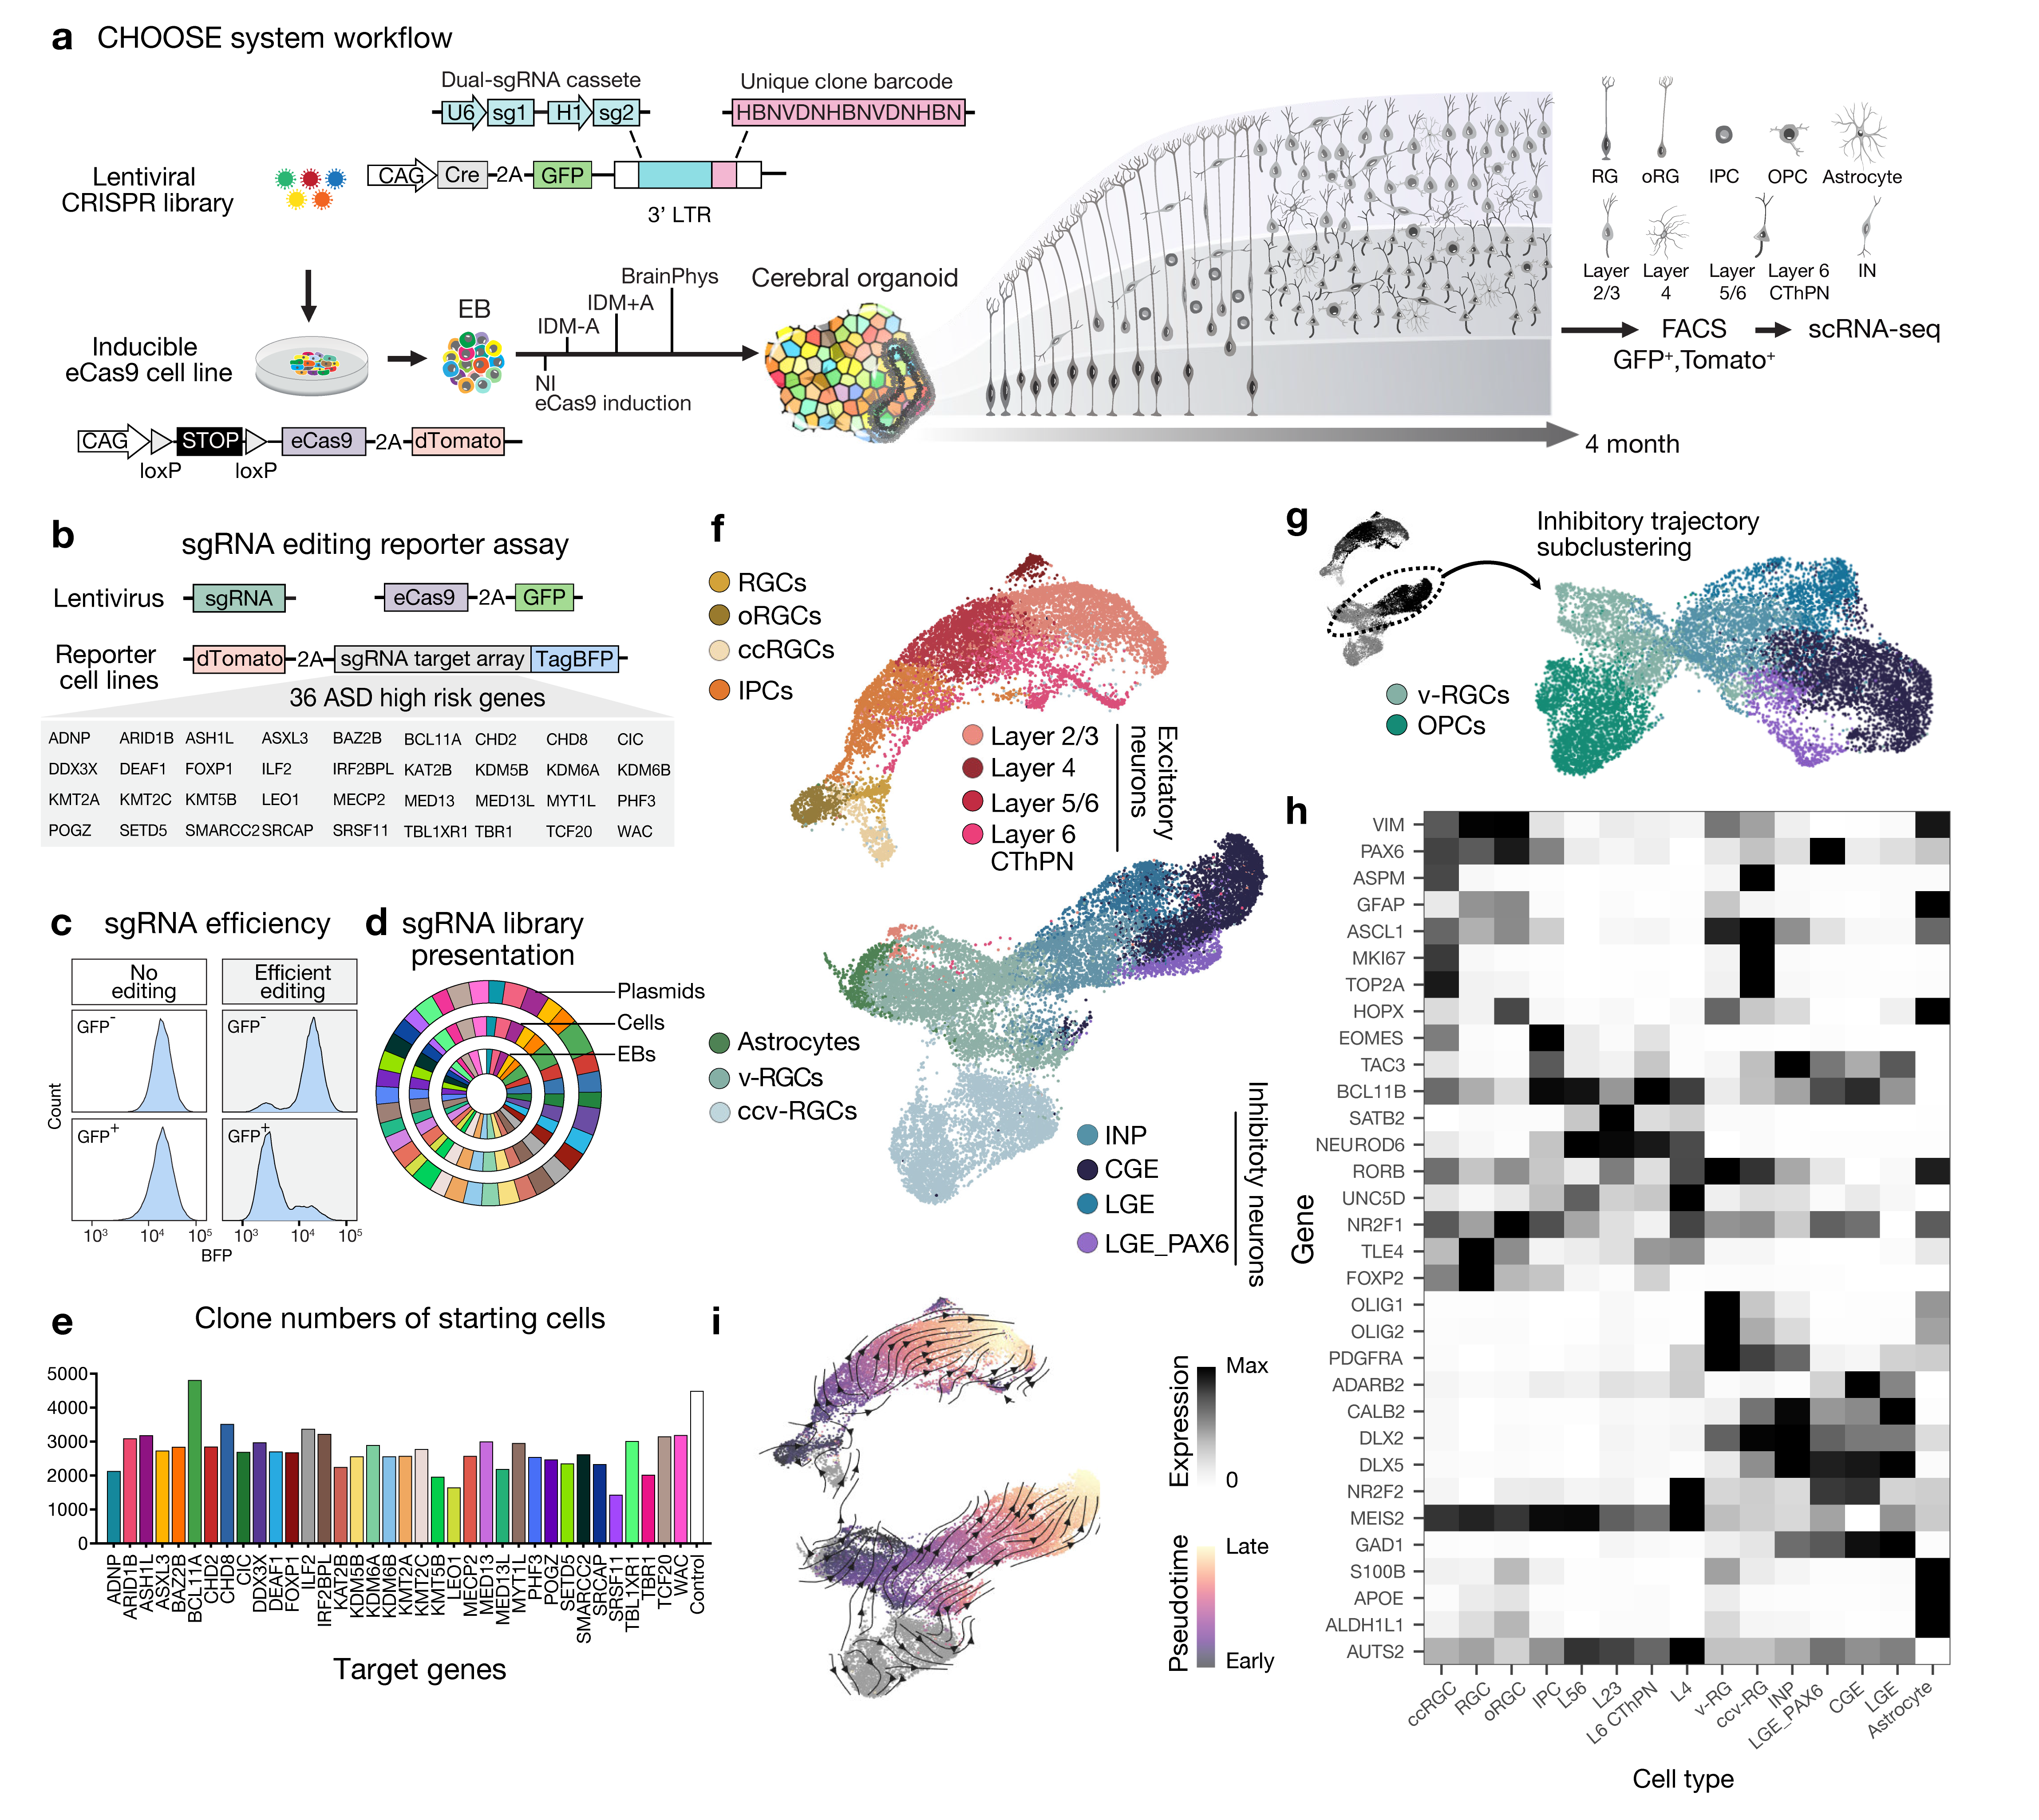
\includegraphics[width=\textwidth]{figures/asd/Figure_1}
    \caption{\textbf{The CHOOSE system for multiplexed screening of ASD risk genes in human cerebral organoids.}
    a, CHOOSE system overview. Barcoded dual-sgRNA cassette located within the 3’ LTR of the lentivirus. b, Reporter assay to test gRNA efficiencies for 36 ASD risk genes. c, Editing efficiencies of gRNAs determined by flow-cytometry. Plots show examples of gRNAs with no or efficient editing. d, sgRNA sequence read distributions of gRNAs sequenced from the ASD plasmid library, lentivirus infected hESCs, and EBs at day 5. e, Numbers of clones from the starting hESCs for each perturbation used to generate mosaic cerebral organoids. f, UMAP embedding of the scRNA-seq dataset containing dorsal and ventral telencephalon trajectories. g, Subclustering and UMAP embedding of the ventral telencephalon trajectory excluding astrocytes and ccv-RGC to annotate OPC clusters. h, Heatmap shows the expression of marker genes in different cell types. i, RNA velocity and velocity pseudotime inference in dorsal and ventral trajectories to show developmental directions.}
    \label{fig:asd1}
\end{figure}

\topparagraph{Single-cell loss-of-function screening in clonally barcoded organoids}
Single-cell RNA sequencing (scRNA-seq) is a high-throughput method for analyzing cellular heterogeneity of complex tissues. To establish an organoid system that enables CRISPR perturbations with single-cell transcriptomic readout, we made use of a human embryonic stem cell (hESC) line that expresses an enhanced specificity SpCas9 (eCas9) with significantly reduced off-target effects and is controlled by an upstream loxp stop element13 (Fig. 1a). To regulate the eCas9 induction, we engineered a lentiviral vector to deliver a 4-hydroxytamoxifen (4-OHT)-inducible CRE recombinase and a dual single-guide RNA (sgRNA) cassette (Fig. 1a). In this cassette, two sgRNAs targeting the same gene are expressed under the U6 or H1 promoter. The dual-gRNA is located within the 3’ long terminal repeat (LTR) of the lentiviral vector and is thus transcribed by RNA polymerase II to be captured by scRNA-seq assays14. To ensure efficient generation of loss-of-function alleles, we determined the editing efficiency of the candidate sgRNAs for each target gene using a flow cytometry-based gRNA reporter assay (Fig. 1b, Extended Data Fig. 1a). In this assay, a pre-assembled array of gRNA-targeting sequences is fused with TagBFP and is transduced in 3T3 cells to generate reporter cell lines. sgRNA and eCas9 are then delivered to the reporter cell lines by lentiviruses. Successful genome editing causing frameshift mutations leads to the loss of BFP fluorescence, allowing us to quantitatively evaluate gRNA efficiency in a large cell population (Fig. 1c, Extended Data Fig. 1b, c). Using our reporter assay, we selected efficient sgRNA pairs for 36 ASD genes (Extended Data Fig. 1d, e, Table 1).  
We cloned sgRNA pairs individually and pooled them equally to construct a lentiviral plasmid library. To ensure that the lentiviral integration frequency is limited to one per cell, we used a low infection rate of 2.5\%15 (Extended Data Fig. 2a-c). Importantly, the development of human brain tissues exhibits generation of cell clones with highly variable sizes both in vivo and in vitro13,16. To monitor the clonal complexity of the founder cells, we introduced a unique clone barcode (1.4 X 107 possible combinations) for each dual-sgRNA cassette to label individual lentiviral integration events (Fig. 1a, Extended Data Fig. 3a-c). Our analysis showed that the homogeneous distribution of the gRNAs presented in the plasmid library and in hESCs at the time of infection and was also maintained after the formation of embryoid bodies (EBs) (Fig. 1d). In addition, for each gene perturbation, we obtained an average of 2,770 unique clones, which we used to generate mosaic EBs (Fig. 1e). Altogether, we established a highly efficient and controlled pooled screening system with high clonal complexity in the organoid. 

\topparagraph{CHOOSE cerebral organoids generate a high diversity of telencephalic cell types} 
Cortical abnormalities are a key pathological feature of ASD6,17. Many ASD risk genes related to transcriptional regulation and chromatin remodeling pathways are crucial for cortical development18,19. However, it was previously not possible to explore which cell types are affected when and how by these risk genes. We thus sought to leverage our methodology to explore loss-of-function phenotypes for 36 transcriptional control genes with high causal confidence (SFARI database category 1 genes)5.
We used previously established protocols which reproducibly generate human telencephalon tissues from human pluripotent stem cells20,21 (Extended Data Fig. 4a-c). Single-cell transcriptomic profiling (10X Genomics Chromium) of cerebral organoids at 4 months revealed a large diversity of cell types composing the developing dorsal and ventral telencephalon (Fig. 1f-h, Extended Data Fig. 5a-c; 31 cerebral organoids). We identified progenitor cells with dorsal (PAX6) or ventral (ASCL1, OLIG2) origins. In the dorsal telencephalon trajectory, we identified radial glial cells (RGCs), cycling RGs (ccRGCs; ASPM), outer radial glial cells (oRGCs; HOPX) and intermediate progenitor cells (IPCs; EOMES). Dorsal progenitors differentiated into excitatory neurons of specific layer identities, including layer 5/6 neurons (L5/6; BCL11B), layer 6 cortical thalamic projection neurons (L6 CThPN; FOXP2, TLE4)22,  layer 4 neurons (L4; RORB, UNC5D, NR2F1)23,24 and layer 2/3 neurons (L2/3; SATB2). Progenitors from the ventral telencephalon differentiated into interneuron precursor cells (INPs; DLX2), which generated interneurons with lateral ganglionic eminence (LGE) origin (LGE-IN; MEIS2), or caudal ganglionic eminence (CGE) origin (CGE-IN; NR2F2)25. Interestingly, we found a cluster of interneurons expressing MEIS2 and strong PAX6 (LGE\_PAX6), which transcriptionally resembles mouse olfactory bulb precursors, and was recently reported to be redirected to white matter specifically in primates26. In addition to neuronal populations, we also identified glial cell populations including astrocytes (S100B, APOE, ALDH1L1) and oligodendrocyte precursor cells (OPC; OLIG2, PDGFRA) (Fig. 1f, g). RNA velocity analysis27 {Bergen NatBiotech 2020} revealed general developmental trajectories from neural progenitor cells to neuronal populations in both the dorsal and ventral telencephalon (Fig. 1i). Taken together, our scRNA-seq dataset of 4-month-old cerebral organoids recapitulates diverse telencephalic cell types that are present in the developing human brain. 

\topparagraph{Perturbing ASD risk genes depletes dorsal IPCs and enriches ventral RGCs}
The presence of the large cellular diversity detected in our organoids allows us to systematically assess, compare, and categorize the effects of perturbations on cell fates. Using targeted amplification and hemi-nested emulsion PCR, we first recovered sgRNA information and assigned 28,344 cells to unique sgRNAs (Methods, Extended Data Fig. 5d, e). With a Cochran-Mantel-Haenszel test stratified by library, we then measured the differential abundance of overall cell populations from dorsal (D) versus ventral (V) telencephalon (hereafter referred to as dorsal and ventral lineage, respectively), as well as of each individual cell type in perturbations versus control (non-targeting sgRNAs) (Fig. 2a, Extended Data Fig. 6). 
We first detected significant changes in the ratio of dorsal to ventral (D-V) lineage (orange to purple, Fig. 2a, left) for 24 perturbations. Interestingly, in most perturbations (21/24) a lowered D-V ratio was detected. On the level of cell types, we detected abundance changes for 21 perturbations (red to blue, Fig. 2a, right) with at least one cell type affected (CMH-test, FDR < 0.05). For example, perturbation of KMT2C led to an overall depletion of the dorsal lineage and enrichment of the ventral lineage, whereas 8 perturbations specifically targeted one cell type without affecting the others, such as ADNP (L2/3 enrichment), MED13L (L2/3 depletion), ILF2 (CGE\_IN enrichment), and DDX3X (CGE\_IN depletion). Perturbations of LEO1 and TCF20 caused an enrichment of L4 neurons, which is a cell population critical for rapid sensory response that serves as the first level of sensory signal processing in cortical neurons28. This is consistent with the fact that sensory and in particular auditory and visual processing concerns are one of the prevalent ASD symptoms29. 
Within the dorsal lineage, we identified depletion of IPCs as a strong convergent effect (Fig. 2a, ARID1B, BCL11A, CHD2, KAT2B, KMT2C, MECP2, MED13, PHF3, SETD5, TBL1XR1), whereas within the ventral lineage, progenitor cells (v-RGCs and ccv-RGCs) and INPs were among the most affected cell populations with an enrichment in most perturbations (e.g. CIC, CHD2, MED13, PHF3 and TBL1XR1). Interestingly, perturbations of three BAF complex members ARID1B, BCL11A and SMARRC2, all lead to an enrichment of v-RGCs, suggesting a critical role of the BAF complex in regulating the cell fate specification of ventral lineages. With respect to ventral telencephalic neurons, we detected LGE-IN enrichment in 7 perturbations, while 3 perturbations caused CGE-IN changes with either a depletion or enrichment effect, indicating an interneuron subtype-specific response to ASD genetic perturbations during development. Beyond neuronal lineages, we found that astrocytes were affected by 2 perturbations with opposite outcomes (enrichment in DEAF1 and depletion in LEO1 perturbations). 
Collectively, the CHOOSE system allowed us to simultaneously investigate the effects of numerous ASD genes on cell fate determination. We found that progenitor populations, including dorsal IPCs and ventral RGCs, are among the most affected cell types, which indicates that ASD pathology could already emerge as early as the neural progenitor stage.  

\begin{figure}[t!]
    \centering
	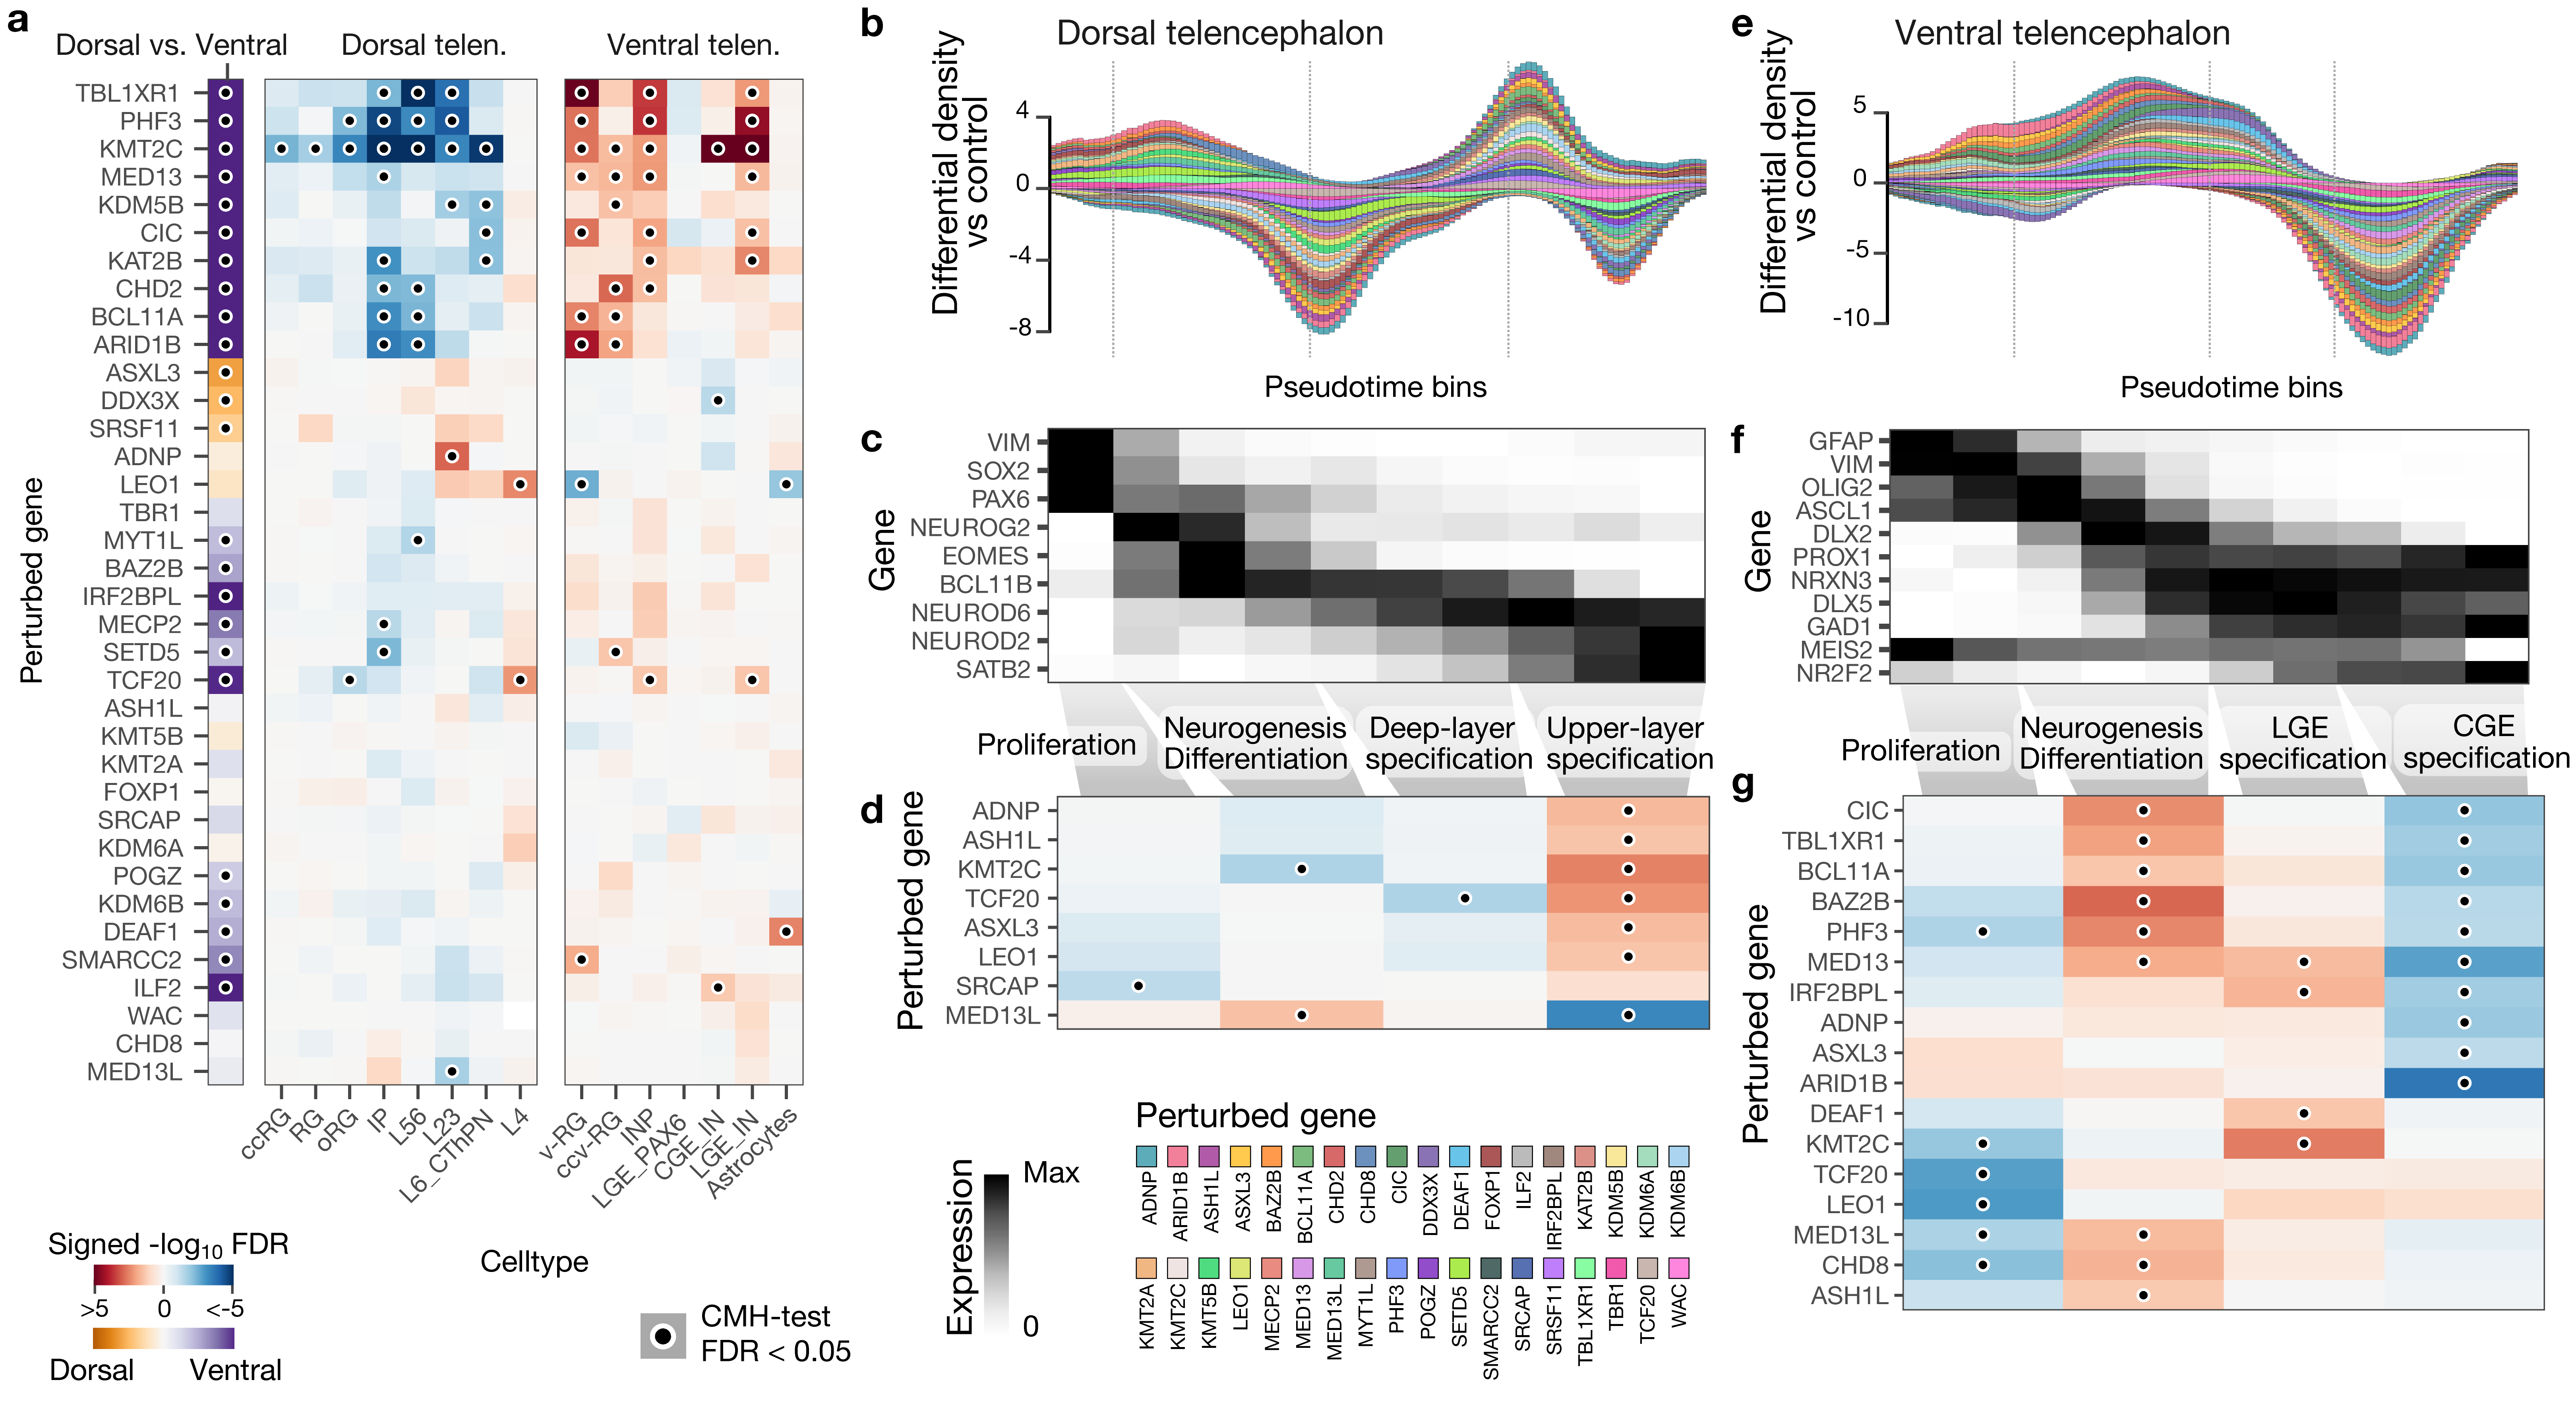
\includegraphics[width=\textwidth]{figures/asd/Figure_2}
    \caption{\textbf{Cell type and developmental process-specific effects of perturbations of ASD risk genes.}
    a, Heatmap shows enrichment of gRNAs versus control in the dorsal versus ventral lineage (left, purple to orange) and individual cell types (middle and right, blue to red). Colors indicate the sign of the log odds ratio multiplied by the -log10 FDR-corrected p-value of a CMH test stratified by library (signed -log10 FDR). b, e, Accumulative differential density of perturbations versus control across a binned pseudo-temporal axis. Each color represents one perturbation. c, f, Heatmaps show the expression of genes used to define developmental stages. d, g, Heatmaps show enrichment of gRNAs in annotated developmental stages for each trajectory.}
    \label{fig:asd2}
\end{figure}

\topparagraph{Perturbing ASD risk genes impairs upper-layer neuronal specification and ventral progenitor differentiation} 
scRNA-seq captures transcriptional dynamics in developing tissues and therefore allows the analysis of cell state transitions {Trapnell NatBiotech 2014} 27 . Using RNA velocity and gene expression patterns, we first defined developmental stages along both the dorsal and ventral telencephalic trajectory covering progenitor proliferation (VIM), onset of neurogenesis (dorsal: NEUROG2; ventral: ASCL1), differentiation (dorsal: BCL11B, NEUROD6; ventral: ASCL1, DLX2, OLIG2), and neuronal subtype specification (dorsal: NEUROD2, NEUROD6, BCL11B, SATB2; ventral: MEIS2, NR2F2, DLX5) (Fig.2c-f). We then calculated the differential density for cells of each perturbation versus control along a binned pseudo-temporal axis within the dorsal and ventral telencephalic trajectory, respectively (Fig. 2b, e, Extended Data Fig. 7). 
The developmental stage-based differential testing provides additional resolution on the effects of perturbations on cell states. For example, in the dorsal trajectory, we found an accumulative high density of perturbed cells in an early stage of upper layer specification, as indicated by decreasing BCL11B and increasing SATB2 expression (Fig. 2b, c). Differential abundance tests revealed that perturbations of ASH1L, ASXL3, and TCF20 were enriched in the upper layer specification stage (Fig. 2d) despite the fact that we did not detect differential abundance of upper layer neurons when comparing to all cell types (Fig. 2a). Thus, the combined analyses of cell states and developmental progression favor the hypothesis that perturbations of these genes cause accelerated upper layer neurogenesis. Additionally, analyses of the ventral trajectory show an enriched density at the stages of neurogenesis and differentiation caused by multiple perturbations (high DLX2 and OLIG2 expression), suggesting that this developmental process is susceptible to ASD genetic perturbations (Fig. 2e-g). Interestingly, other perturbations which did not cause cell type compositional changes nonetheless affected specific processes along a developmental trajectory. For example, disrupting the chromatin remodeler SRCAP results in reduced dorsal neural stem cell proliferation, which is consistent with a recently identified role of SRCAP in stem cell self-renewal30(Fig. 2d). 
Overall, our perturbation-specific characterizations of differential abundance of cell types as well as of stages along developmental trajectories together create a unique resource to delineate ASD high-risk gene loss-of-function phenotypes.

\begin{figure}[b!]
    \centering
	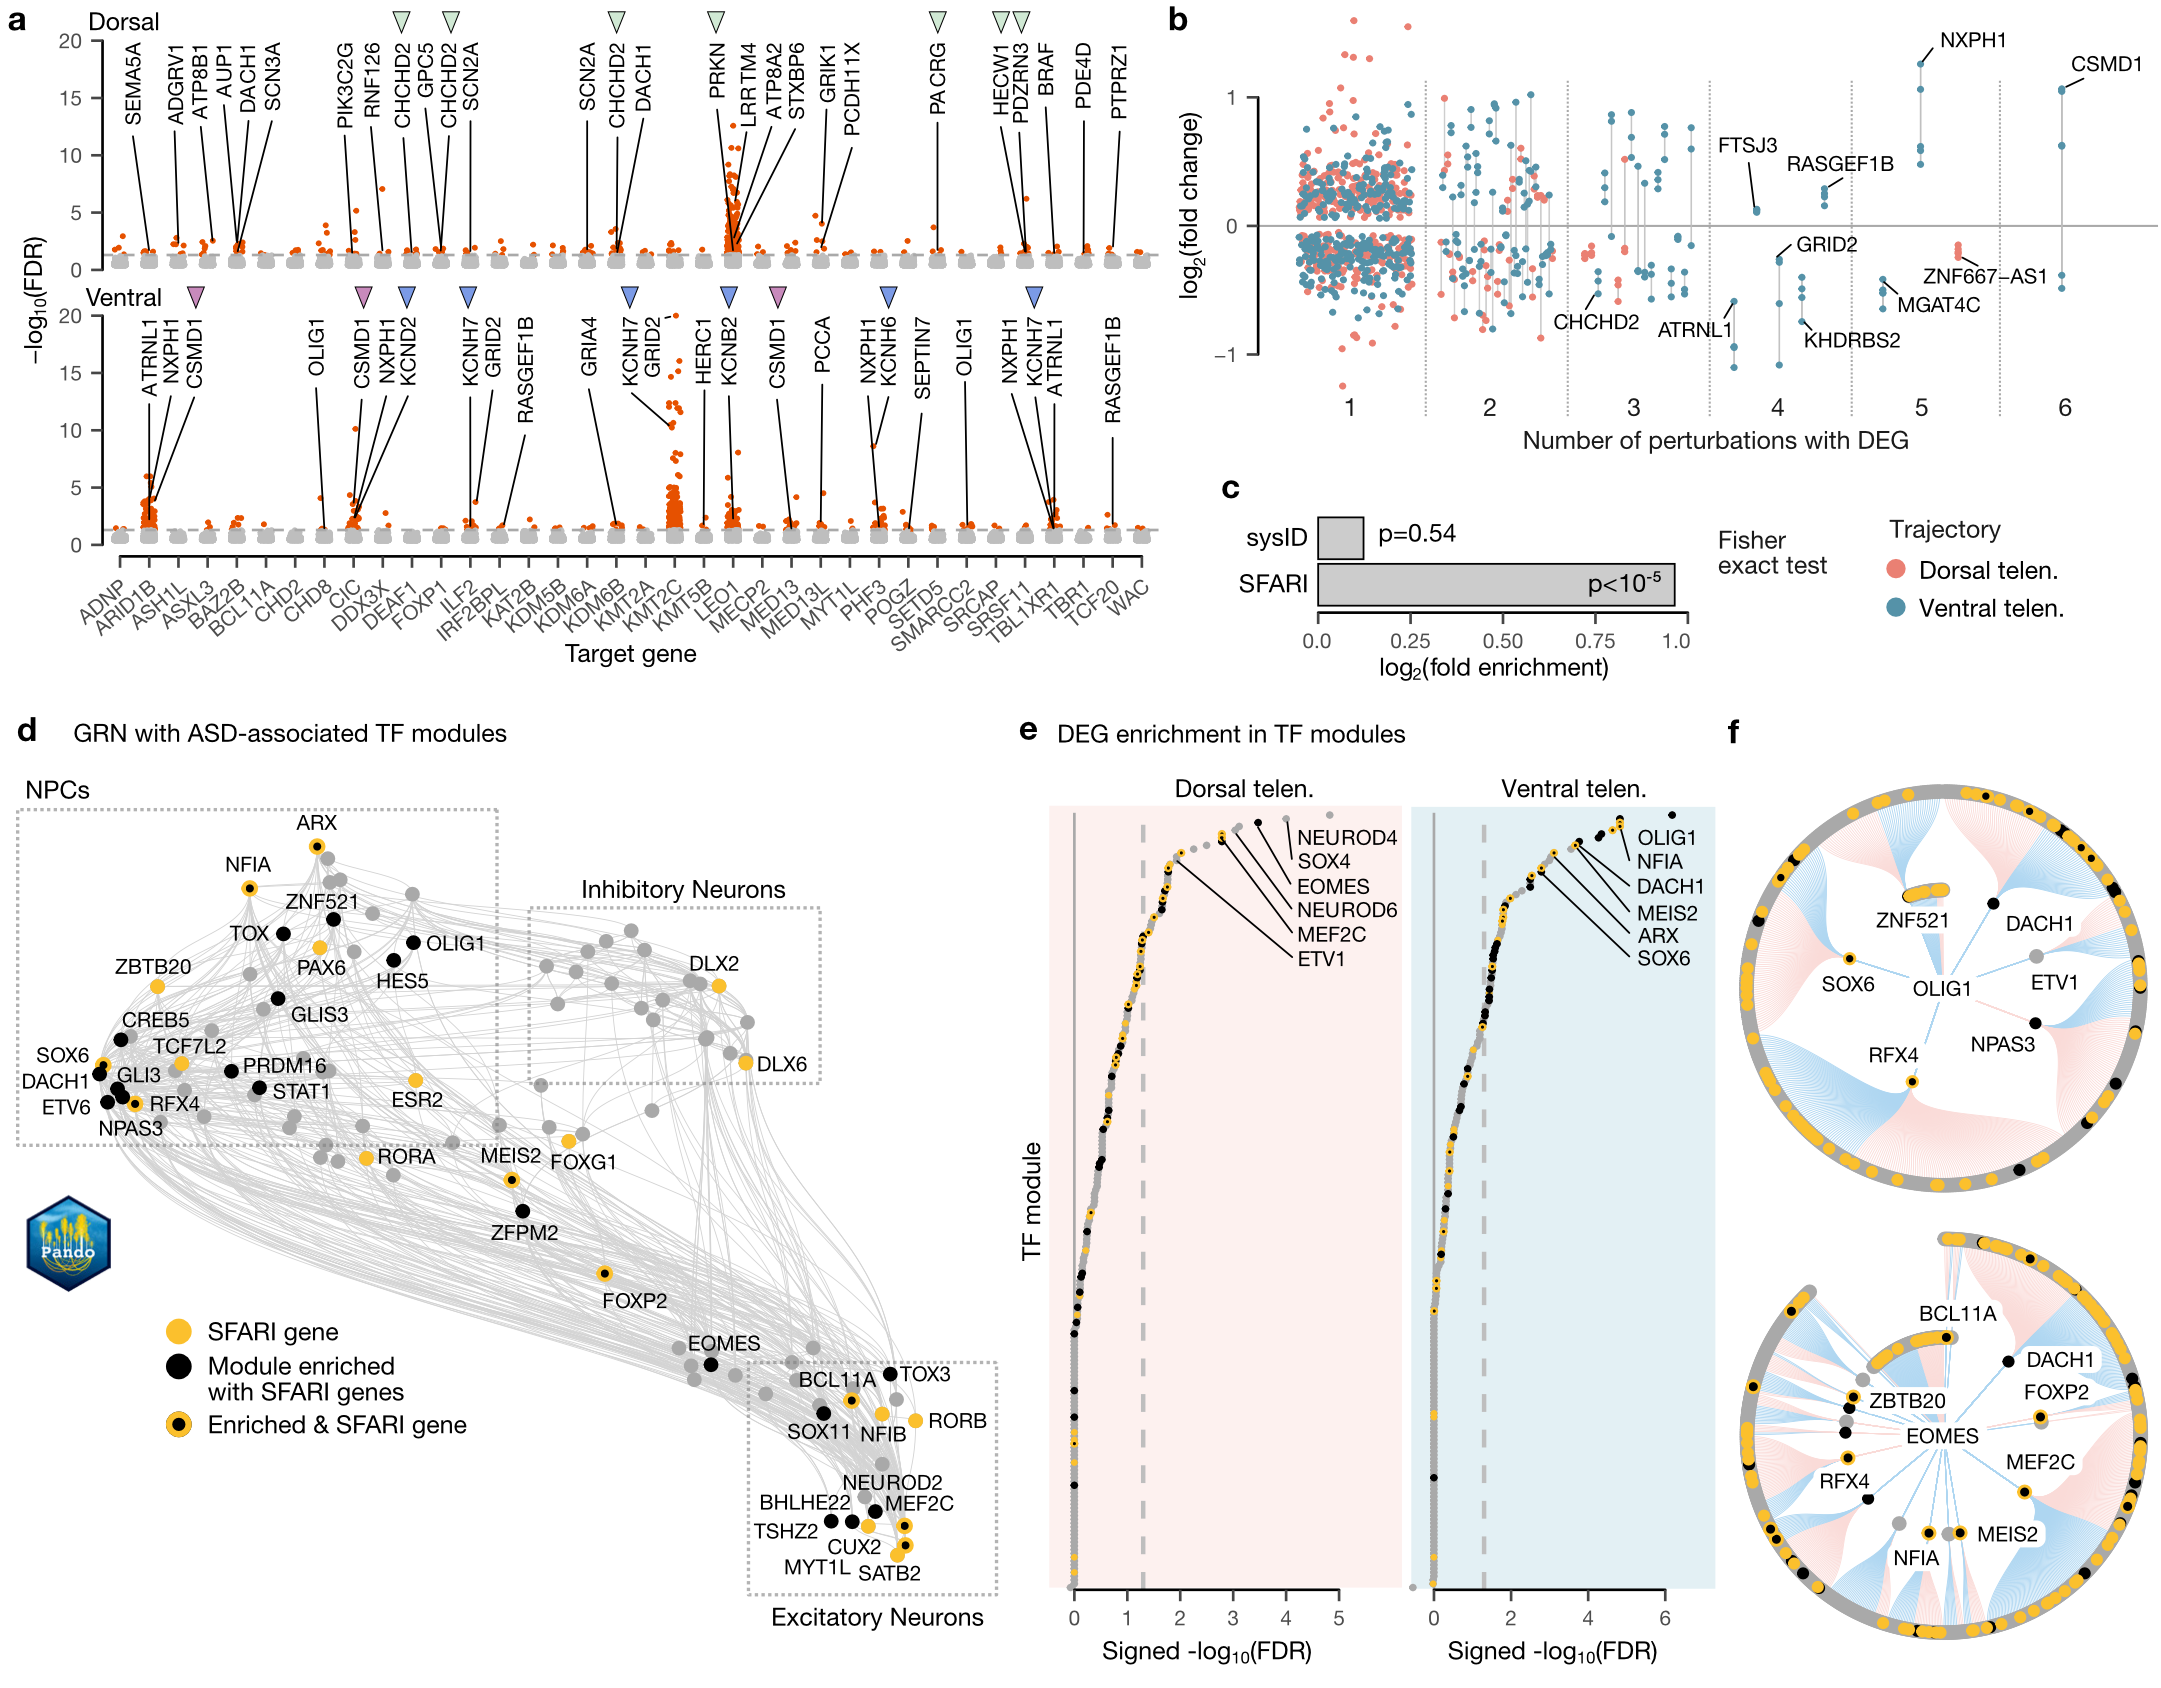
\includegraphics[width=\textwidth]{figures/asd/Figure_3}
    \caption{\textbf{Dysregulated gene expression and regulatory networks caused by perturbations of ASD risk genes.}
    a, Manhattan plots show DEGs detected in dorsal (top) and ventral (bottom) trajectories from each genetic perturbation. Green arrowheads indicate genes associated with PD (CHCHD2, PRKN, PACRG) or the ubiquitin system (PRKN, HECW, PDZRN3). Blue arrowheads indicate genes encoding VGKCs. b, Jitter plot shows frequency of DEGs detected from all perturbations separated by dorsal (blue) and ventral (orange) trajectories. Points belonging to the same gene are connected with a gray line. c. Enrichment test of TOP-DEGs (top 30 DEGs from each perturbation) in ID (sysID database) or ASD (SFARI database) genes. The p-value was obtained from a Fisher exact test. d, GRN of 4-month-old cerebral organoids inferred by Pando showing developmental TF modules constructed based on their co-expression and interaction strengths. ASD-specific TF modules are highlighted in yellow (SFARI genes) and/or black (regulator of SFARI genes). e, Lolliplots show CHOOSE-DEG enriched TF modules in dorsal and ventral trajectories. f, Circular GRN plots show primary and secondary targets of OLIG1 and EOMES. ASD-specific TF modules are highlighted in black/yellow as described above.}
    \label{fig:asd3}
\end{figure}

\topparagraph{CHOOSE identifies lineage-specific dysregulated genes}
To further assess molecular changes caused by each perturbation, we performed differential gene expression analysis comparing each perturbation to control within dorsal and ventral lineages and detected 885 differentially expressed genes (DEGs) in total (Fig. 3a, top, dorsal lineage; bottom, ventral lineage; Supplementary Data 1). We ranked DEGs by detection frequency and discovered that certain genes, or gene families, are identified in multiple perturbations (Fig. 3b). Interestingly, in the dorsal lineage, perturbations of DEAF1, FOXP1 and KDM6B, all lead to the down-regulation of CHCHD2 (Fig. 3a), a gene encoding a mitochondrial coiled-coil-helix-coiled-coil-helix domain containing protein and associated with Parkinson’s disease (PD)31. CHCHD2 was also found to be downregulated in both excitatory and inhibitory neuronal lineages in postmortem brain tissues from several autism patients32. Additionally, 4 other PD or ubiquitin proteasome pathway associated genes are dysregulated, including PRKN (LEO1 perturbation), PACRG (SETD5 perturbation), HECW1 and PDZRN3 (SRSF11 perturbation) (Fig. 3a). Of note, ubiquitin genes have been identified to cause autism33. Our findings support the role of a dysregulated ubiquitin proteasome system in the pathophysiology of ASD during development. In the ventral lineage, the most frequently detected DEG is the adhesion molecule CSMD1 (Fig. 3a, b), which is upregulated by ARID1B, CIC, MED13, and PHF3 perturbations, and downregulated by LEO1 and KMT2C perturbations.
Ion channel deficiency has been implicated in NDDs and is strongly associated with neurological conditions such as epilepsy34. We found that genes encoding voltage-gated potassium channels (VGKCs), including KCNB2, KCND2, KCNE5, KCNH6, and KCNH7, are differentially expressed in at least one of seven perturbations (ARID1B, CIC, ILF2, KMT2C, LEO1, PHF3, TBL1XR1) in the ventral lineage (Fig. 3a). VGKCs play an important role in regulating neuronal excitability and have been linked to ASD35. Interestingly, genes related to sodium channels are specifically dysregulated in the dorsal lineage (Fig. 3a, top, SCN2A upregulation in ILF2 and KDM6A perturbations, SCN3A upregulation in BAZ2B perturbation), but not in the ventral lineage. These data suggest a lineage-specific channel dysregulation caused by ASD genetic perturbations. 


\topparagraph{CHOOSE combined with GRN inference from single-cell multiome data identifies ASD-specific transcription regulatory modules}
When combining the DEGs from all perturbations, we found that they were significantly enriched in risk genes associated with ASD (SFARI database, 1031 genes; ~2-fold enrichment, p < 10-5; Fig. 3c, d; Supplementary Data 1). Interestingly, however, we did not observe enrichment in risk genes for other neurodevelopmental disorders such as intellectual disability (ID; SysID database, 936 primary ID genes; Fig. 3c) indicating that certain biological processes and developmental regulatory programs are specifically susceptible to ASD-associated gene perturbations. To explore these potential gene regulatory ‘hubs’, we first generated single-cell multiomic data including single cell transcriptome and chromatin accessibility modalities from 4-month-old cerebral organoids (Extended Data Fig. 8a-d). Using Pando36, we could harness these multimodal measurements to infer a gene regulatory network of the developing telencephalon and extract sets of genes regulated by each transcription factor (TF modules) (Extended Data Fig. 8e,f). We visualized this TF network using a UMAP embedding {McInnes 2018 https://arxiv.org/abs/1802.03426; Becht 2019 NatBiotech}, which revealed distinct groups of TFs active in NPCs (PAX6, GLI3, OLIG1), inhibitory neurons (DLX2, DLX6) and excitatory neurons (NEUROD2, NFIB, SATB2) as well as regulatory interactions between the TFs (Fig. 3e). 
To test whether regulatory sub-networks indeed exist at which ASD risk genes accumulate, we tested all TF modules for enrichment with SFARI genes. We found significant enrichment for a set of 40 TFs (adjusted Fisher test p-value < 0.01, >2-fold enrichment) (Extended Data Fig. 8g), among which 14 TFs are ASD risk genes (e.g. NFIA, BCL11A, MEF2C), and others are regulators of ASD risk genes (e.g. OLIG1, DACH1, EOMES) (Fig. 3e). All TF regulatory modules enriched in SFARI genes together form an ASD-specific sub-GRN.
Next, we assessed the transcriptomic effect of ASD genetic perturbations in the context of the inferred GRN. We performed enrichment tests on perturbation-induced DEGs (CHOOSE-DEGs) from dorsal and ventral telencephalic cells separately. We found that, similar to ASD risk genes, CHOOSE-DEGs were enriched in specific TF modules (Fig. 3f). In the ventral telencephalic cells, OLIG1 and NFIA were most strongly affected, whereas dorsal telencephalon-specific DEGs were most strongly enriched in NEUROD4, SOX4 and EOMES modules. Interestingly, some of the ASD-specific TF modules were among the most strongly enriched in CHOOSE-DEGs, supporting their role in ASD-specific gene dysregulation (Fig. 3f). We finally present gene regulatory subnetworks of OLIG1 and EOMES, two important genes whose regulomes are both enriched in ASD risk genes and strongly affected by ASD genetic perturbations (Fig. 3g). 
Taken together, we have characterized gene expression changes for each genetic perturbation in both dorsal and ventral telencephalon and uncovered novel molecular programs shared between different perturbations. Leveraging GRN inference from single-cell multiomic data, we further identified ASD-specific TF modules during cortical development and critical regulatory hubs underlying the detected gene expression changes.

\begin{figure}[b!]
    \centering
	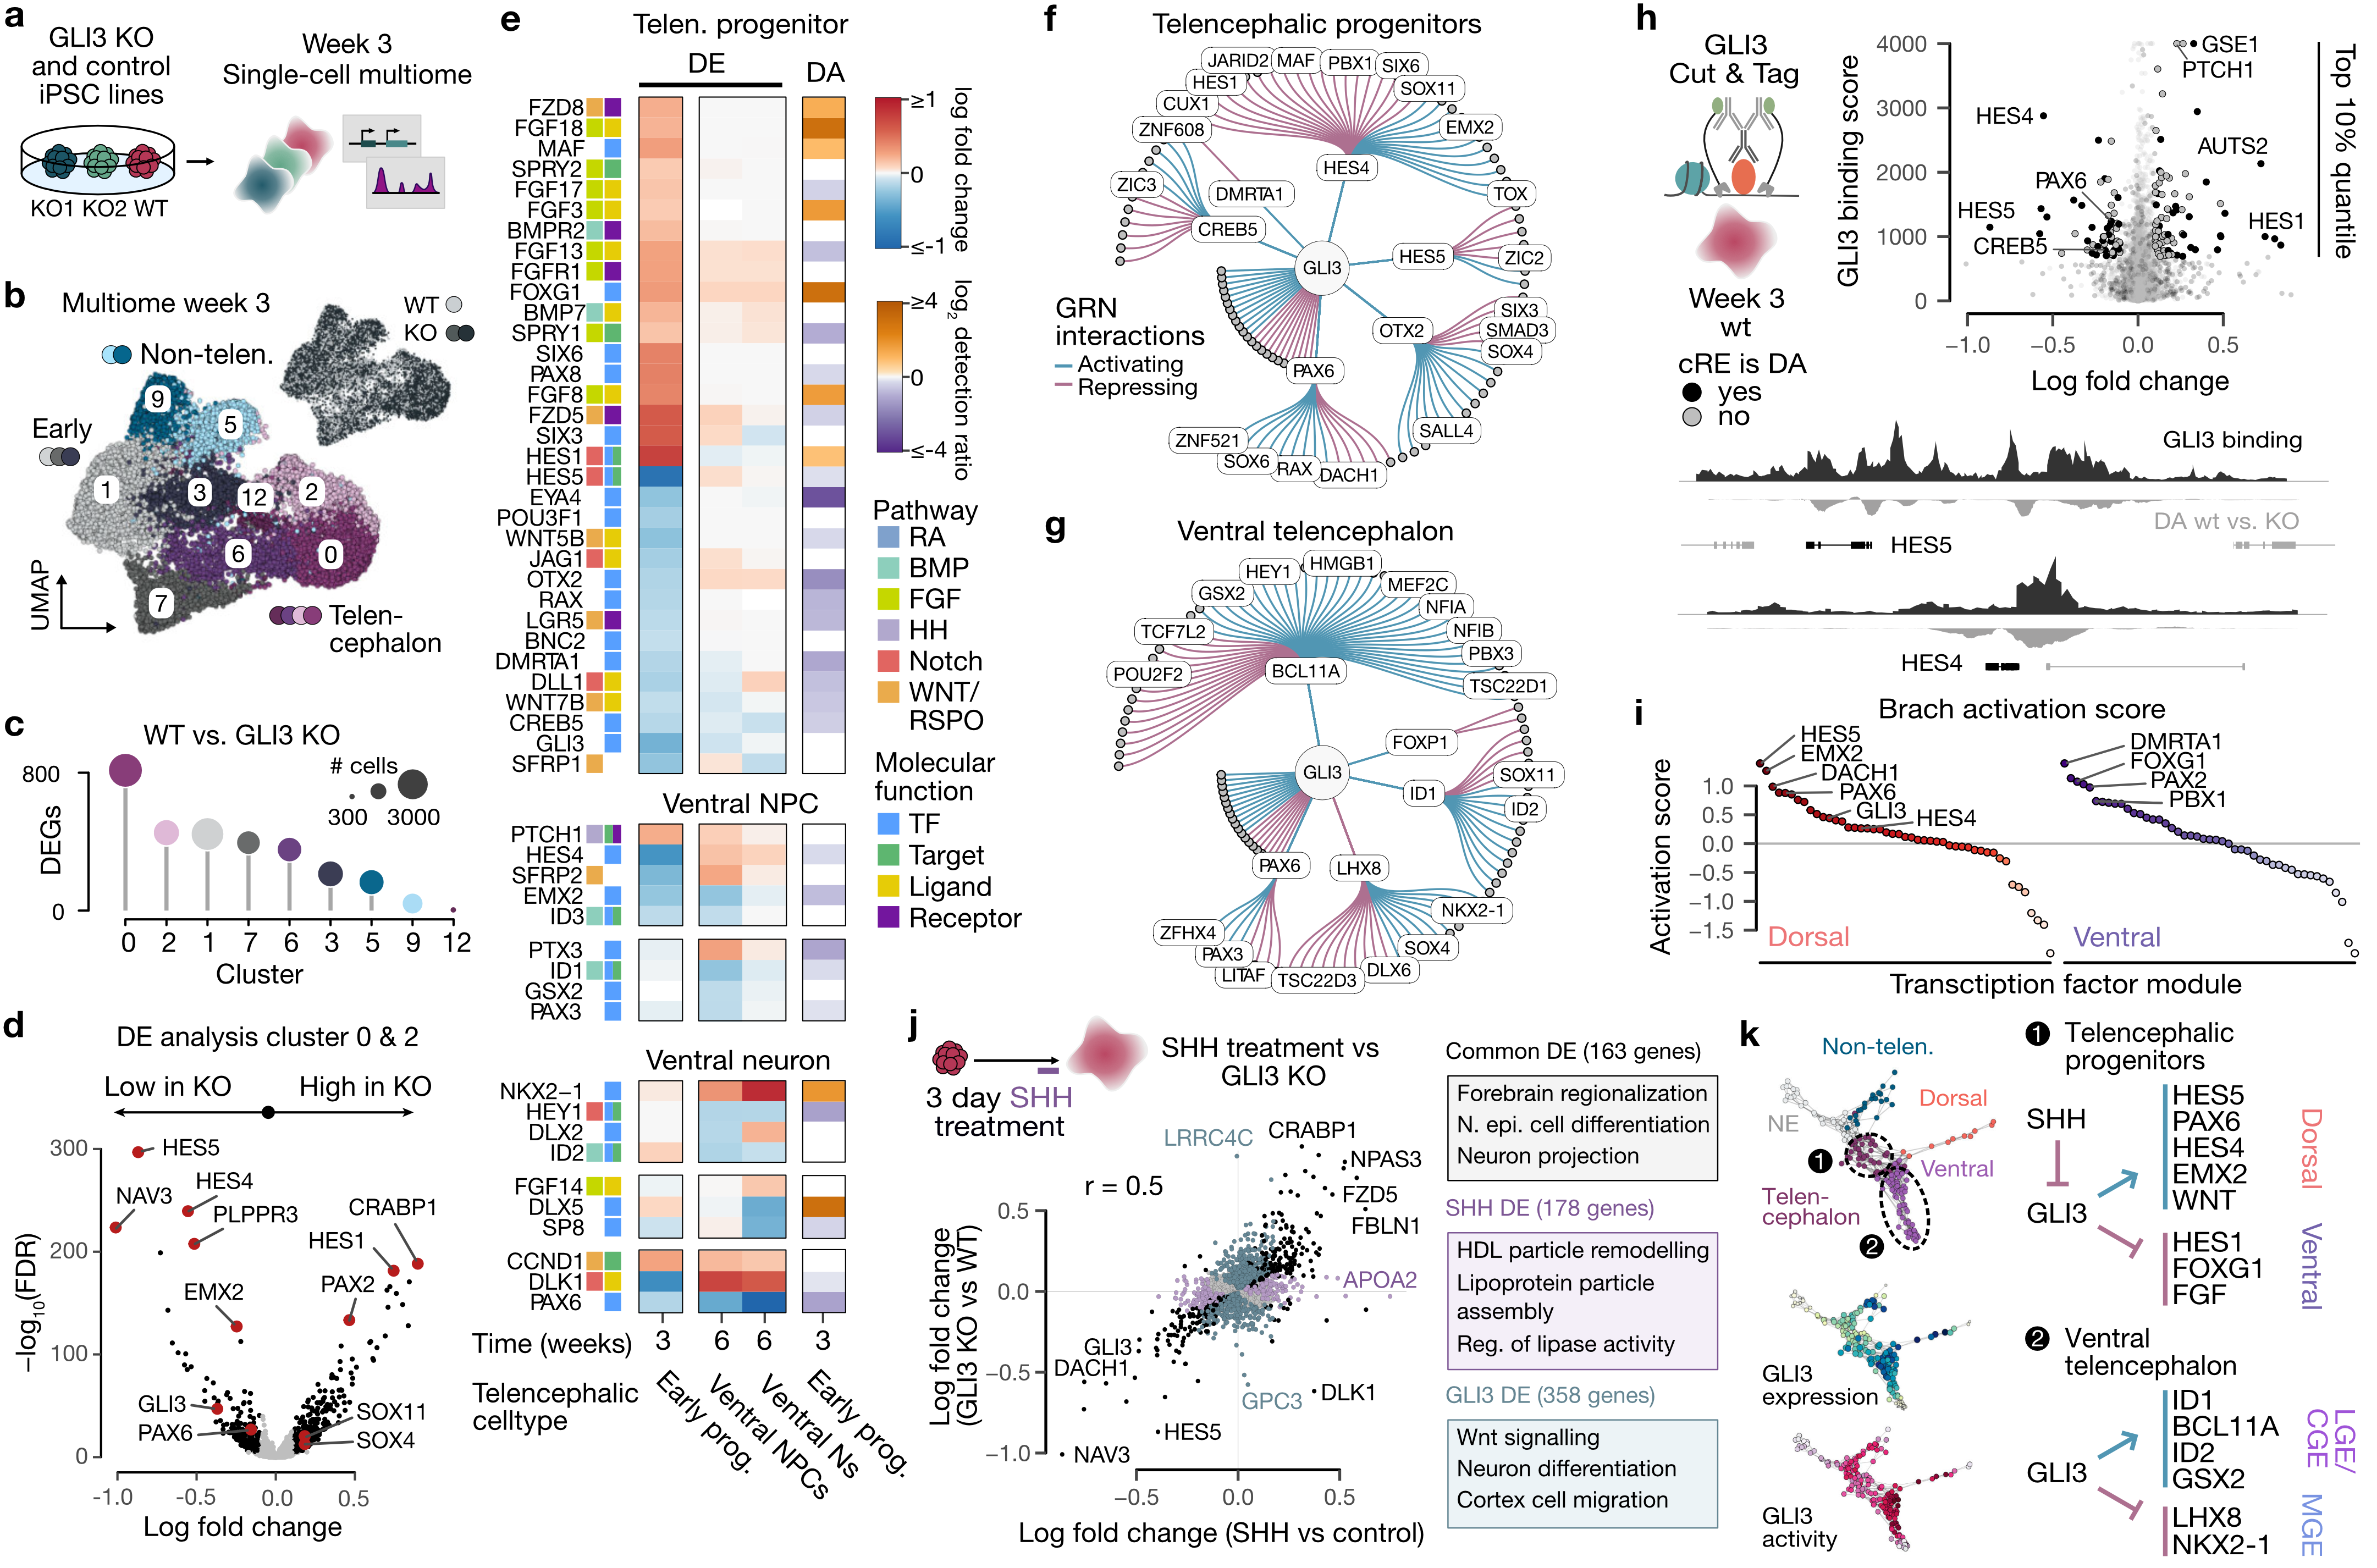
\includegraphics[width=\textwidth]{figures/asd/Figure_4}
    \caption{\textbf{Perturbation of ARID1B increases the transition of v-RGCs to early OPCs.}
    a, Circular projection of terminal fate probabilities shows ventral telencephalon differentiation trajectories. b, Trajectory branches defined by gene expressions of DLX2 (INP), DLX5 (IN), OLIG2 (early OPC) and PDGFRA (late OPC). c, Differential density of cells with ARID1B perturbation versus control. d, Bar graph shows cells within the v-RGCs are positive for DLX2 (68.6\% versus 81.5\%), OLIG2 (19.6\% versus 36.2\%) and both (9.8\% versus 30.6\%) in control versus ARID1B perturbation. e, Box plots showing transition probabilities of control and ARID1B perturbed ventral progenitor cells towards OPCs. Middle line depicts the median; box marks the 25\% and 75\% quantiles. f, Immunohistochemistry for early OPCs (OLIG2) and INPs (DLX2) of day 40 ventralized brain organoids derived from control (c. 220dupG repair) and two ARID1B patient iPSCs. Scale bar, 200 μm. g, Violin plots (all data points and median values) show numbers of cells positive for OLIG2 and/or DLX2. Control, n =108 areas from 13 organoids, 4 batches; ARID1B+/- (c.2201dupG), n = 104 areas from 15 organoids, 4 batches; ARID1B+/- (6q25.3del), n = 94 areas from 15 organoids, 3 batches. One-way ANOVA post hoc Tukey test. ***P<0.01. h, Prenatal magnetic resonance imaging scan and 3D reconstruction of LGE and CGE (marked as GE) from age matched controls and ARID1B patient showing enlarged GE in the patient. Quantified in Extended Data Fig. 10c. Scale bar, 1 cm. I, Diagram showing ARID1B perturbation-induced cellular responses of ventral progenitors.}
    \label{fig:asd4}
\end{figure}

\topparagraph{ARID1B perturbation increases the transition probability of v-RGCs to early OPCs}
Amongst the 36 genes, we found that ARID1B perturbation causes one of the most dramatic enrichments of v-RGCs (Fig. 2a). Interestingly, the OLIG1 regulatory module was also specifically enriched in DEGs caused by ARID1B perturbation (Extended Data Fig. 9). These data intrigued us to further investigate how v-RGCs are affected by ARID1B perturbation. We used Cellrank37 to resolve the developmental trajectories leading to different inhibitory neuron types as well as OPC populations (Fig. 4a). We visualized the terminal fate probabilities for each cell as a circular projection {Velten 2017 NatCellBio}, which revealed a distinct differentiation trajectory from ventral progenitors towards early OPCs (OLIG2, PDGFRA) and a branching of INPs (DLX2) into different inhibitory neuronal fates (DLX5) (Fig. 4b). We found that ARID1B perturbed cells were strongly enriched in the OPC trajectory and had a higher percentage of OLIG2+ v-RGCs (Fig. 4c, d). This is an interesting finding given that OLIG2 is known to regulate progenitor self-renewal at earlier developmental stages and is a master regulator for oligodendrocyte lineage specification in the ventral telencephalon38,39. We then analyzed fate transition probabilities of ventral progenitors and found that ARID1B-perturbed v-RGCs have significantly higher transition probabilities towards early OPC than neuronal fates (Fig. 4e).
Loss-of-function mutations in ARID1B have been identified to cause ID and ASD5,40. To confirm whether our findings are relevant to human disorders, we recruited two patients with ARID1B heterozygous mutations. Patient 1 harbors a nucleotide duplication (c.2201dupG) that results in a frameshift and an early STOP codon, and Patient 2 carries a microdeletion (6q25.3del) that includes exon 8 and the downstream region of the ARID1B locus (Extended Data Fig. 10a, b). We established iPSC lines from both patients and a mutation-corrected cell line for patient 1 as an isogenic control. We then generated cerebral organoids with enriched ventral telencephalon regions by adding patterning factors SAG and IWP2 and investigated the behavior of v-RGCs at day 4041. In organoids from both patients, we observed considerably increased OLIG2+ cells, as well as DLX2+, and DLX2+/OLIG2+ cells compared to the control, which is in line with our previous findings (Fig. 4g). Finally, to further explore the potential consequences of such defects in patients, we analyzed the prenatal brain structure of patient 2 using intra-uterine super-resolution MRI obtained at two gestation stages (GW22 and GW31). 3D reconstruction of the LGE and CGE, sources of ventral telencephalon progenitors, revealed an enlarged volume compared to multiple age-matched controls at both stages (Fig. 4h, Extended Data Fig. 10c). Taken together, the enrichment of v-RGCs and ccv-RGCs (Fig. 2a), the higher transition probability of v-RGCs to early OPCs, and the increased proportion of OLIG2+ cells in our CHOOSE experiment and in organoids generated from two patient iPSC lines, all suggest that ARID1B perturbation leads to abnormal ventral progenitor expansion and aberrant cell fate specification (Fig. 4i). We propose that this translates to the enlarged volume of the LGE and CGE in the ARID1B patient.


\subsection{Discussion}
We have developed the CHOOSE system to characterize the loss-of-function phenotypes of 36 high-risk ASD genes across dozens of cell types spanning early brain developmental stages in human cerebral organoids. Our findings provide a developmental and cell-type specific phenotypic database for ASD high-risk gene loss-of-function research, which will shed light on the disease pathogenesis.
We assessed phenotypes affecting dorsal and ventral telencephalic lineages during brain development. IPCs are transit-amplifying dorsal progenitors which generate neurons for all cortical layers and contribute to the evolutionary expansion of the human cortex42,43. We found that IPCs appeared to be particularly susceptible to ASD genetic perturbations. Interestingly, some of the perturbed genes have previously been suggested to play a role in IPC regulation within a disease context. For example, brain organoids derived from a patient with an MECP2 mutation were shown to have decreased number of IPCs44. 
In the ventral lineage, we identify a strong enrichment of progenitor cells, including v-RGs and ccv-RGs, which are the major progenitor pools differentiating into interneurons and oligodendrocytes38,45. Compared to CGE-INs, which can be depleted or enriched, we found that LGE-INs appeared to be only enriched by perturbations. Our results establish a basis for dissecting the relevance of CGE and LGE-IN dysfunction in ASD pathophysiology, which is important considering recently discovered human-specific CGE and LGE interneuron migration features and function21,26,46.
Additionally, DEG analyses revealed that multiple perturbations impaired the same molecular processes, which may be critical for the development of ASD pathophysiology. For example, we found that specifically in the dorsal lineage, genes related to Parkinson’s disease and the ubiquitin system are frequently dysregulated. Interestingly, parkinsonism features have been reported in older autistic adults47. Our findings further suggest that ubiquitin dysfunction could already be emerging during early development stages. Furthermore, we constructed a GRN underlying telencephalon developmental trajectories and identified ASD-specific regulatory modules in dorsal and ventral lineages. The OLIG1 regulatory module is particularly interesting as many of its downstream targets are ASD risk genes (SFARI database). This regulatory module was previously identified as being important for oligodendrocyte differentiation in the developing human cerebral cortex19. Thus, our findings highlight the involvement of the oligodendrocyte lineage in the development of ASD pathophysiology.
Finally, we discovered that loss of ARID1B, a BAF complex component, leads to an increased transition of ventral progenitors to early OPCs.  Interestingly, the OLIG1 regulatory module is also affected by ARID1B perturbation. The role of the BAF complex in oligodendrocyte generation and maturation has been mainly established by studying one of its components, SMARCA4, which is required for OPC differentiation48. Considering the temporal and cell-type specific expression of each BAF subunit, it would be interesting to investigate how ARID1B or other subunit-mediated chromatin remodelers regulate oligodendrocyte specification and how their dysfunction contributes to neurodevelopmental disorders.
The ability to determine cell-type specific contributions to genetic disorders in a systematic, scalable, and efficient manner will greatly facilitate our understanding of disease mechanisms. As the CHOOSE system provides a robust, precisely controlled screening strategy, we anticipate it will be widely applied beyond brain organoids to study disease-associated genes. 


\subsection{Methods}

\paragraph{Data availability}
Raw sequencing data will be deposited on ArrayExpress. Processed Seurat objects will be deposited on Zenodo and will be made available under restricted access before publication. The Pando R package is available on GitHub: \\
(https://github.com/quadbiolab/Pando) \\
Other custom code used in the analyses is deposited on GitHub: \\ 
(https://github.com/quadbiolab/ASD\_CHOOSE).

\paragraph{Acknowledgements}
We are grateful to the patients and their families for participating in this study. We thank all Knoblich lab members for support and discussions; François Bonnay, Emmanouella Chatzidaki, Oliver L. Eichmüller, Ramsey Najm, and Jaydeep Sidhaye for comments on the manuscript; Mario Nezhyba and Thomas Lendl from the IMP/IMBA Biooptics Facility for technical support; Alexander Vogt and Florentina Drochter from the VBCF NGS facility for scRNA-seq library preparation; the IMBA Stem Cell Core facility for generation of iPSC lines. Work in J.A.K.’s laboratory is supported by a SFARI pilot award (724430), the Austrian Federal Ministry of Education, Science and Research, the Austrian Academy of Sciences, the City of Vienna, and the SFB F78 Stem Cell (F 7803-B). Work in B.T.’s laboratory is supported by the European Research Council (Organomics, B.T.; Braintime, B.T.), the Chan Zuckerberg Initiative DAF, an advised fund of the Silicon Valley Community Foundation (CZF2019-002440), the Swiss National Science Foundation (310030\_192604) and the National Center of Competence in Research Molecular Systems Engineering. A.V. is supported by an EMBO Fellowship (ALTF-1112-2019). J.S.F was supported by a Boehringer Ingelheim Fonds PhD fellowship.

\paragraph{Author contributions}
C.L. and J.A.K. conceived the project and experimental design and secured the funding. C.L., J.S.F., and J.A.K. prepared the manuscript with input from B.T. and all authors. C.L. performed all the experiments and analyzed the data with the help from T.R.B., A.V., A.M.P., and C.E., J.S.F. performed the analysis of scRNA-seq and multiome data under the supervision of B.T., M.S. and G.K. performed patient diagnosis and analyzed MRIs, C.M. generated iPSC lines under the supervision of N.S.C., U.E. provided sgRNA predication.   
 
\paragraph{Corresponding authors}
Correspondence and requests for materials should be addressed to C.L., B.T., or J.A.K.

\paragraph{Competing interests}
J.A.K. is on the supervisory and scientific advisory board of a:head bio AG (https://aheadbio.com) and is an inventor on several patents relating to cerebral organoids. The authors declare that they have no conflicts of interest.	



\clearpage

\subsection{Supplement}
\beginsupplement

\begin{figure}[h!]
    \centering
	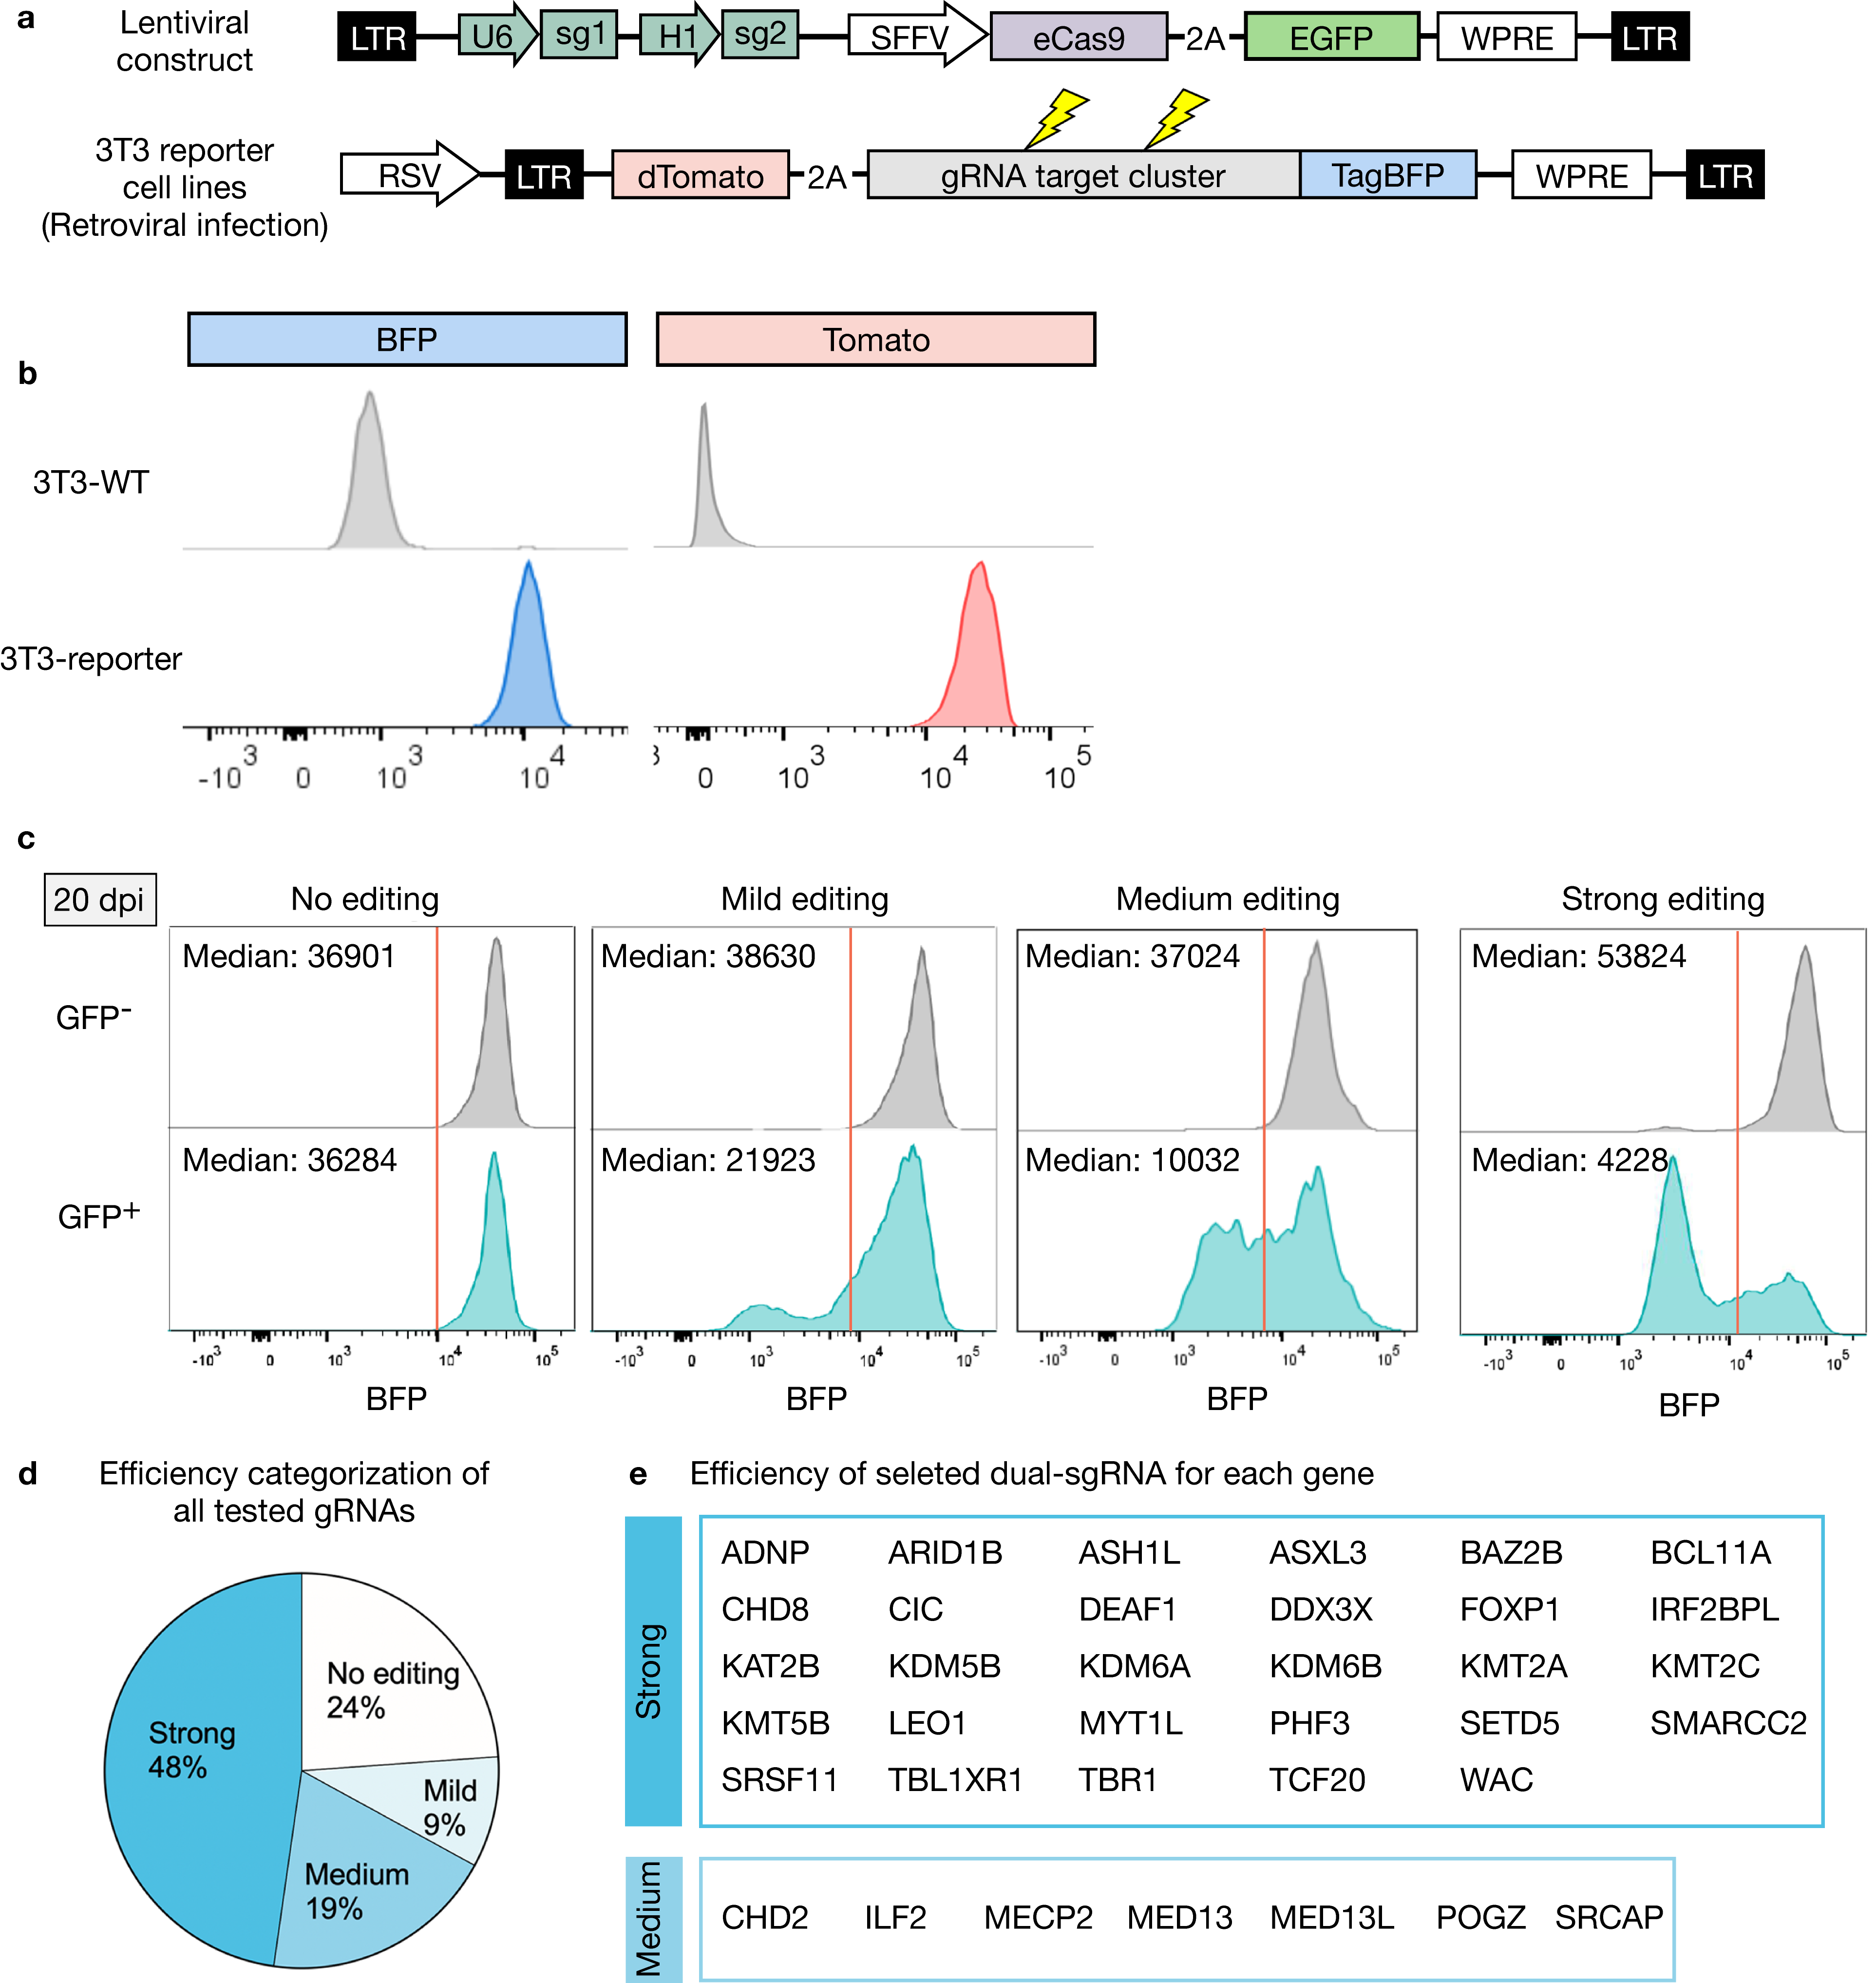
\includegraphics[width=\textwidth]{figures/asd/Figure_S1}
    \label{fig:asdS1}
    \caption{\textbf{A gRNA reporter assay to determine gRNA efficiency.} a, Diagram of the lentiviral construct delivering dual-sgRNA cassette and eCas9 under the spleen focus forming virus (SFFV) promotor. Lentivirus Infected cells are labeled with GFP. Retroviral transduction is used to generate 3T3 cell lines. A pre-assembled array of gRNA-targeting sequences is fused with TagBFP. b, Flow cytometry graph shows a 3T3 reporter cell line is positive for both BFP and Tomato. After lentiviral infection, transduced cells (GFP+) and internal control cells (GFP-) are subjected to FACS-based analysis at 20 dpi. Efficient editing causing frameshift mutations lead to the loss of BFP fluorescence. c, Four dual-sgRNA examples show no (0-10\% reduction), mild (10-45\% reduction), medium (45-75\% reduction) and strong editing efficiency (> 75\% reduction) at 20 dpi, respectively, based on median fluorescence intensity. d, 98 pairs of gRNAs were tested and categorized into four groups. e, Editing efficiency of selected paired gRNAs from 36 ASD genes.}
\end{figure}



\begin{figure}[h!]
    \centering
	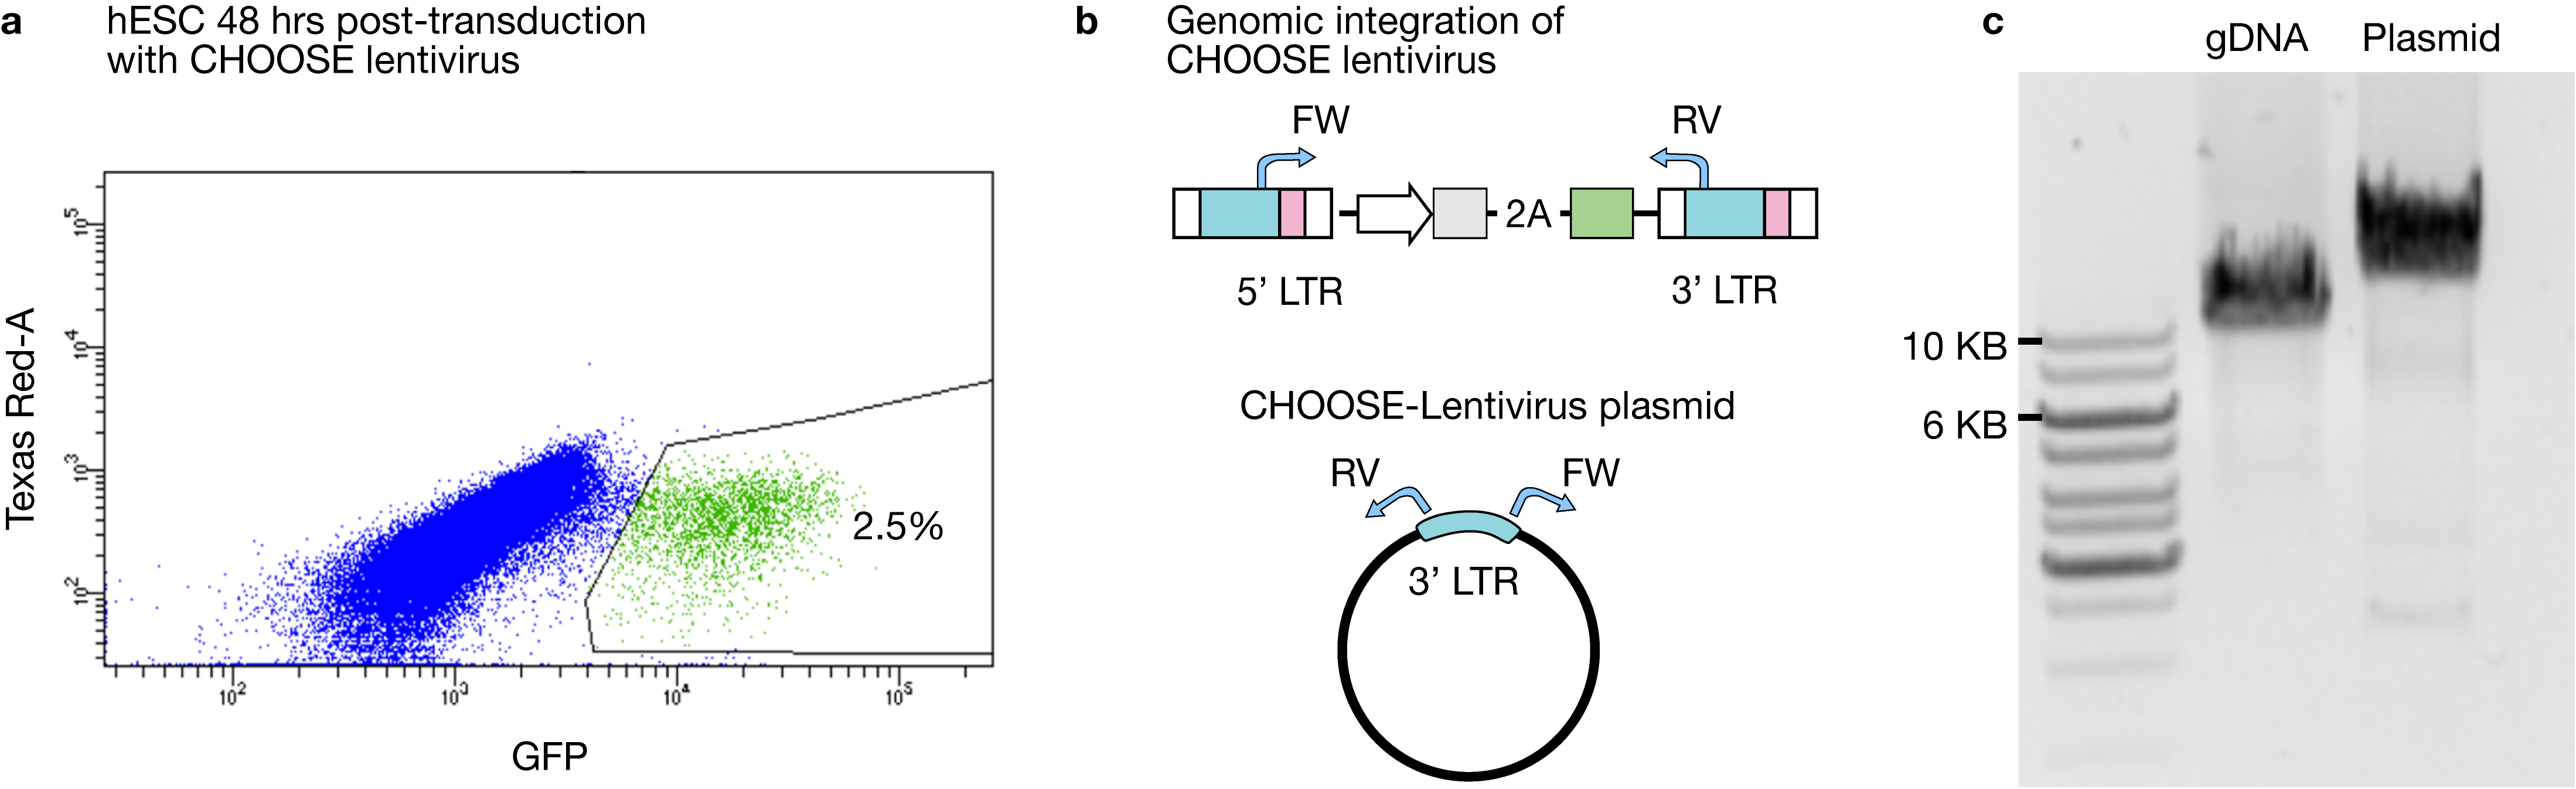
\includegraphics[width=\textwidth]{figures/asd/Figure_S2}
    \label{fig:asdS2}
    \caption{\textbf{Infection and integration of CHOOSE lentivirus on hESCs.} 
    a, Infection rate of CHOOSE lentivirus on hESCs determined by flow-cytometry. Infected cells are positive for GFP. b, Top diagram shows the duplication of the dual-sgRNA cassette after the lentiviral integration into the host genome. FW and RV are paired primers used to demonstrate the successful integration of the lentivirus. The primers amplify specific regions of the genomic DNA extracted from lentivirus-infected hESCs, and the lentiviral plasmid. c, Gel electrophoresis analysis showing 12 kb and 13 kb bands detected from gDNA and plasmid respectively.}
\end{figure}


\begin{figure}[h!]
    \centering
	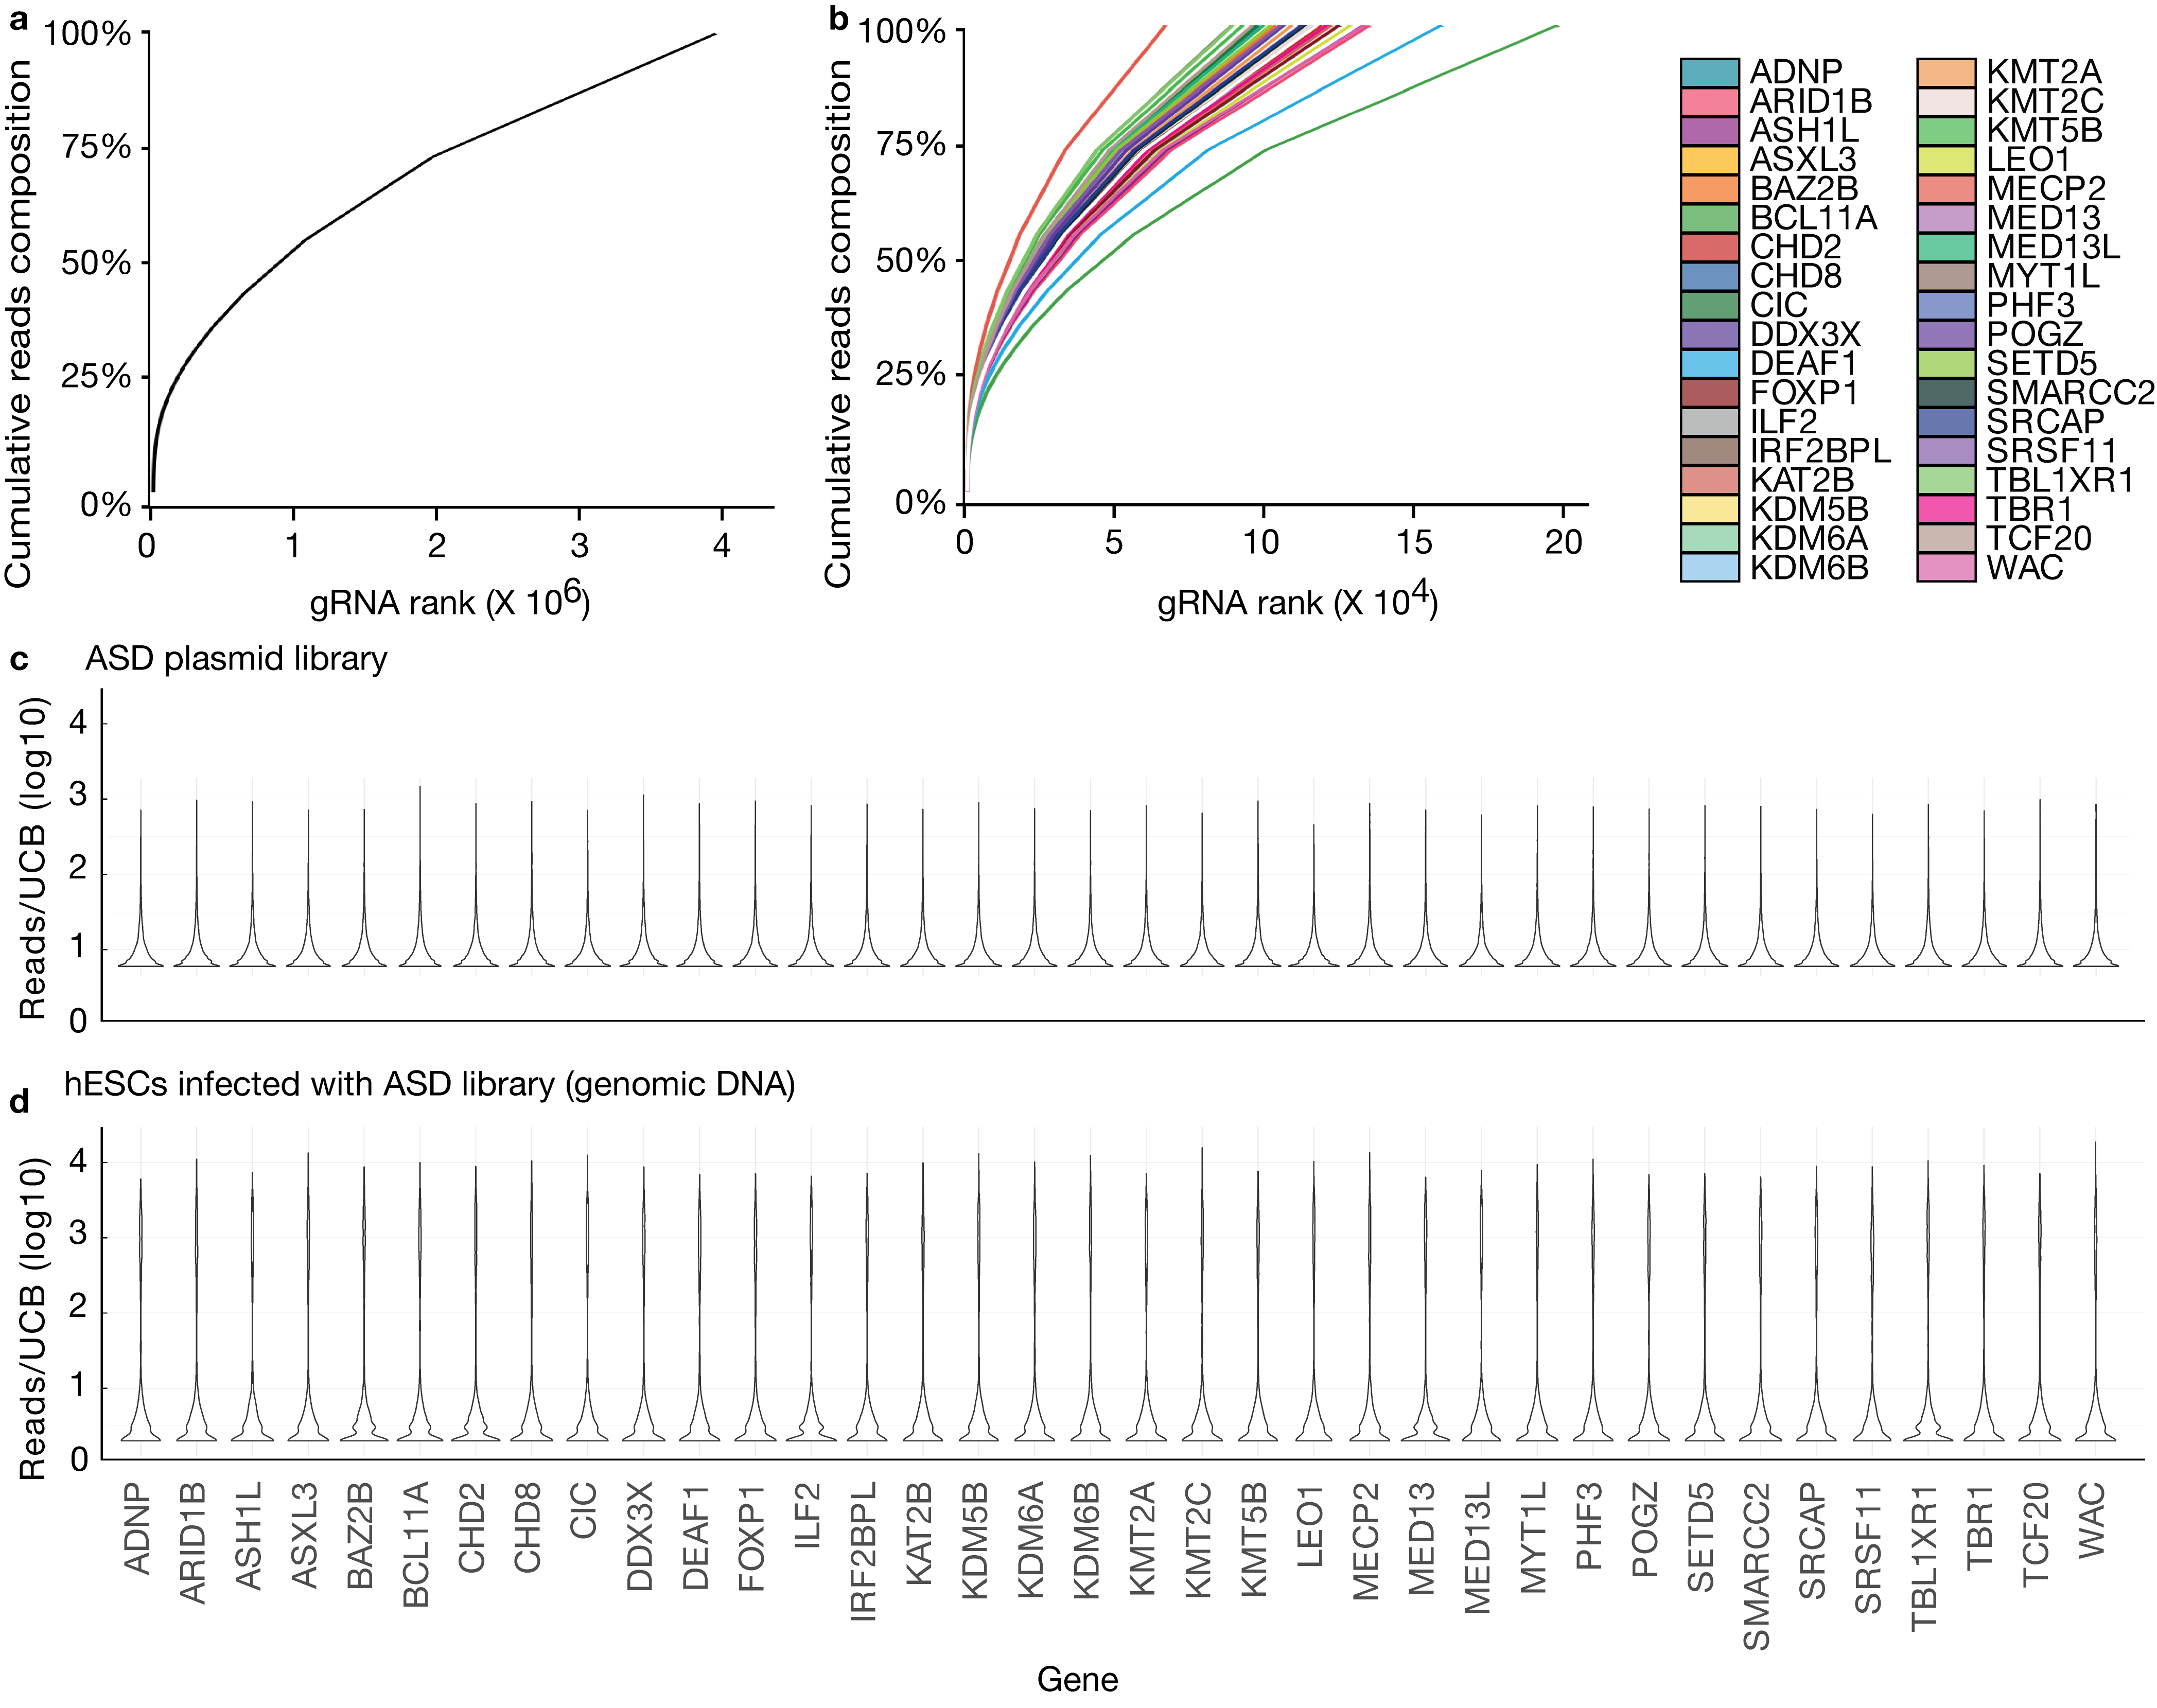
\includegraphics[width=\textwidth]{figures/asd/Figure_S3}
    \label{fig:asdS3}
    \caption{\textbf{Clone barcode diversity of the CHOOSE library.} 
    a, Plot shows cumulative fraction of uniquely barcoded gRNA cassettes from the CHOOSE ASD plasmid library. b, Plot shows cumulative fraction of uniquely barcoded gRNA cassettes separated by each target gene from the plasmid library. c,d, Reads distribution for each barcoded gNRA cassette from the  plasmid library (c) and from genomic DNA (d) extracted from the hESCs infected by lentivirus. UCB, unique clone barcode.}
\end{figure}



\begin{figure}[h!]
    \centering
	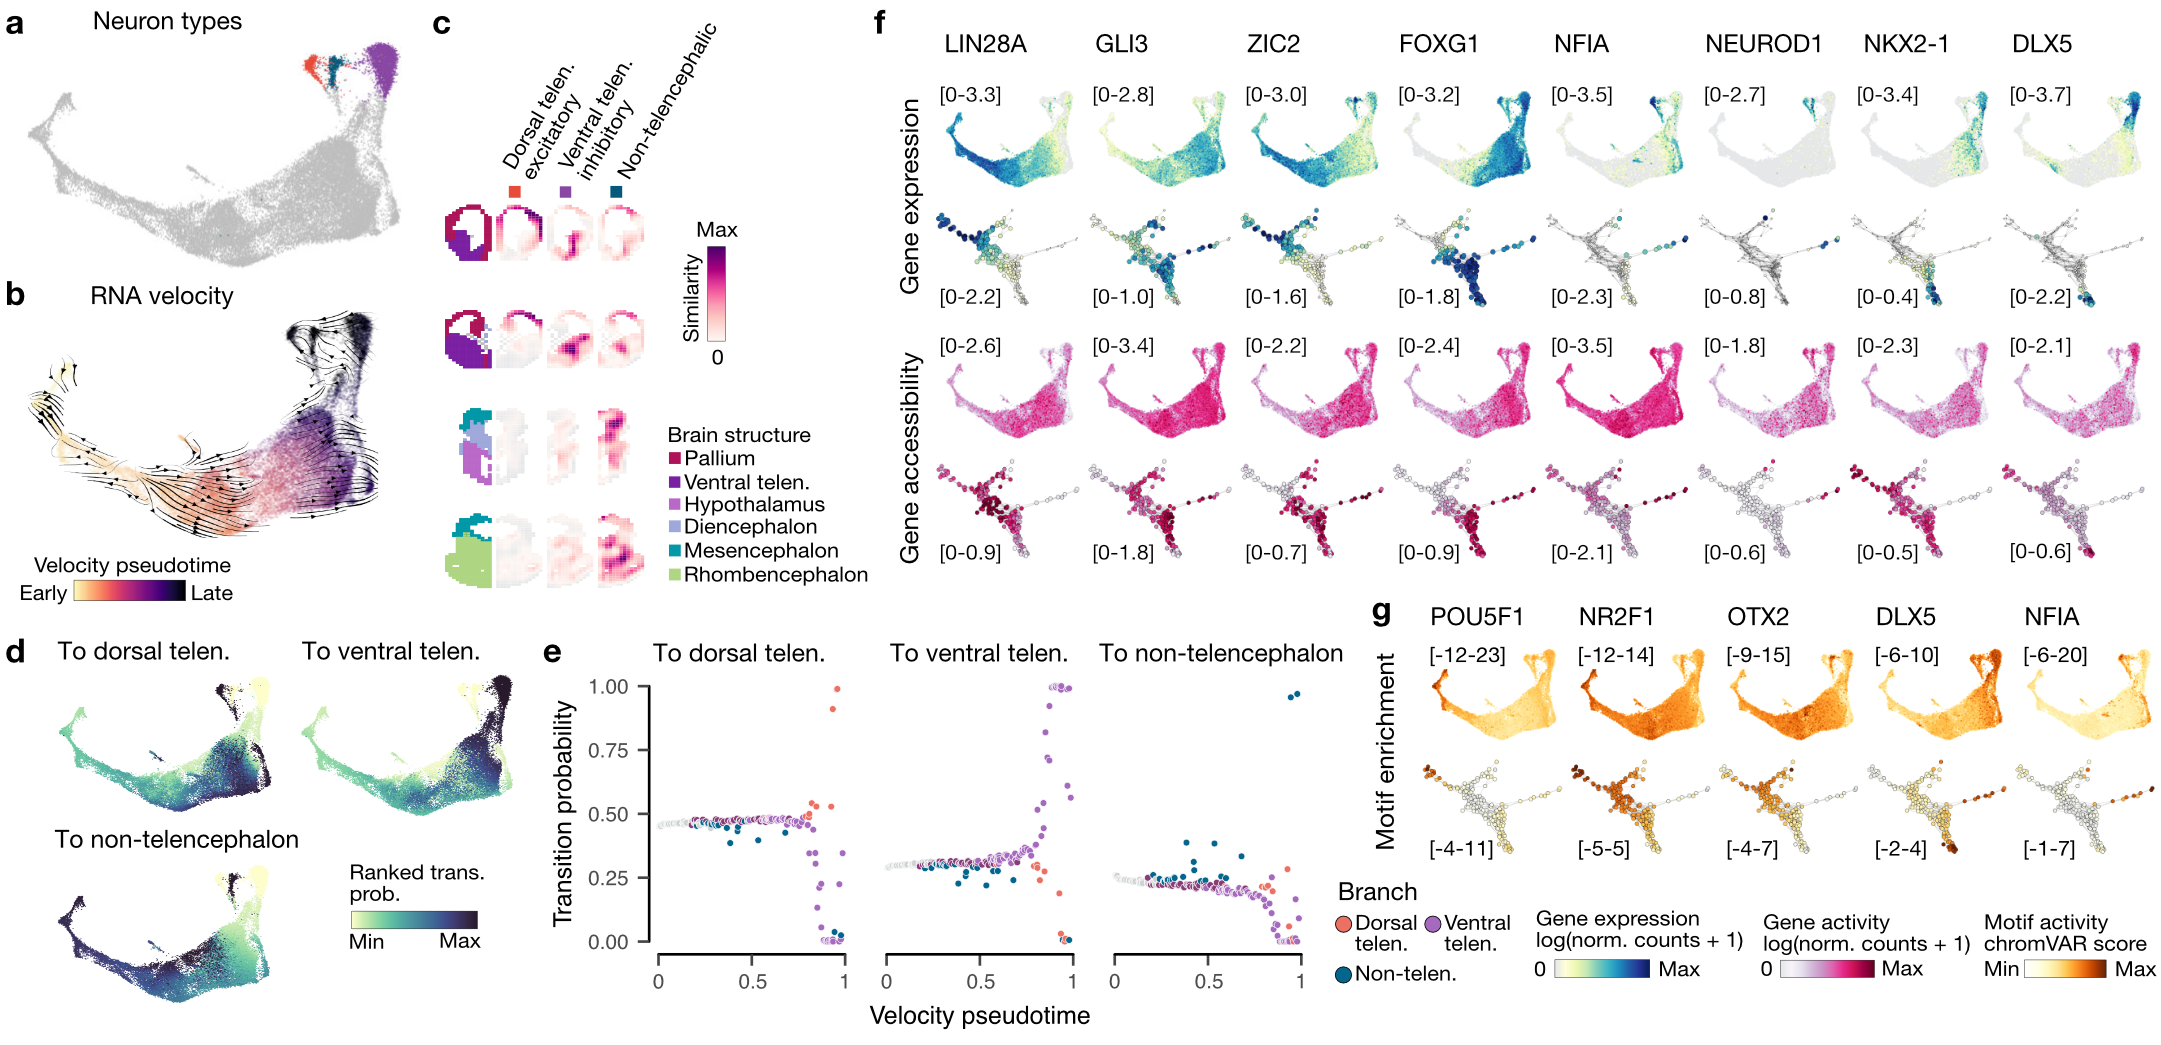
\includegraphics[width=\textwidth]{figures/asd/Figure_S4}
    \label{fig:asdS4}
    \caption{\textbf{Generation of cerebral organoids using the CHOOSE system.} 
    a, Schematic showing the protocol used for generating cerebral organoids. 4-OHT was added to induce eCas9 expression at day 5. A short 3-day CHIR treatment was applied from day 12-14. Culture medium was switched to Brainphys after day 60 for advanced neuronal maturation. Tissues are collected at day 120 and subjected to scRNA-seq assays. b, ESCs were infected by lentivirus and GFP positive cells were collected to make EBs. Microscopic images show the overall morphology and GFP expression of brain organoids overtime. Top, bright-field; Bottom, GFP fluorescence. c. Immunohistochemical staining of cerebral organoids at day 24. GFP labels cells infected with lentivirus and Tomato is a reporter for eCas9 expression. SOX2 is a marker for progenitor cells. FOXG1 is a marker for tissues with telencephalon identity.}
\end{figure}



\begin{figure}[h!]
    \centering
	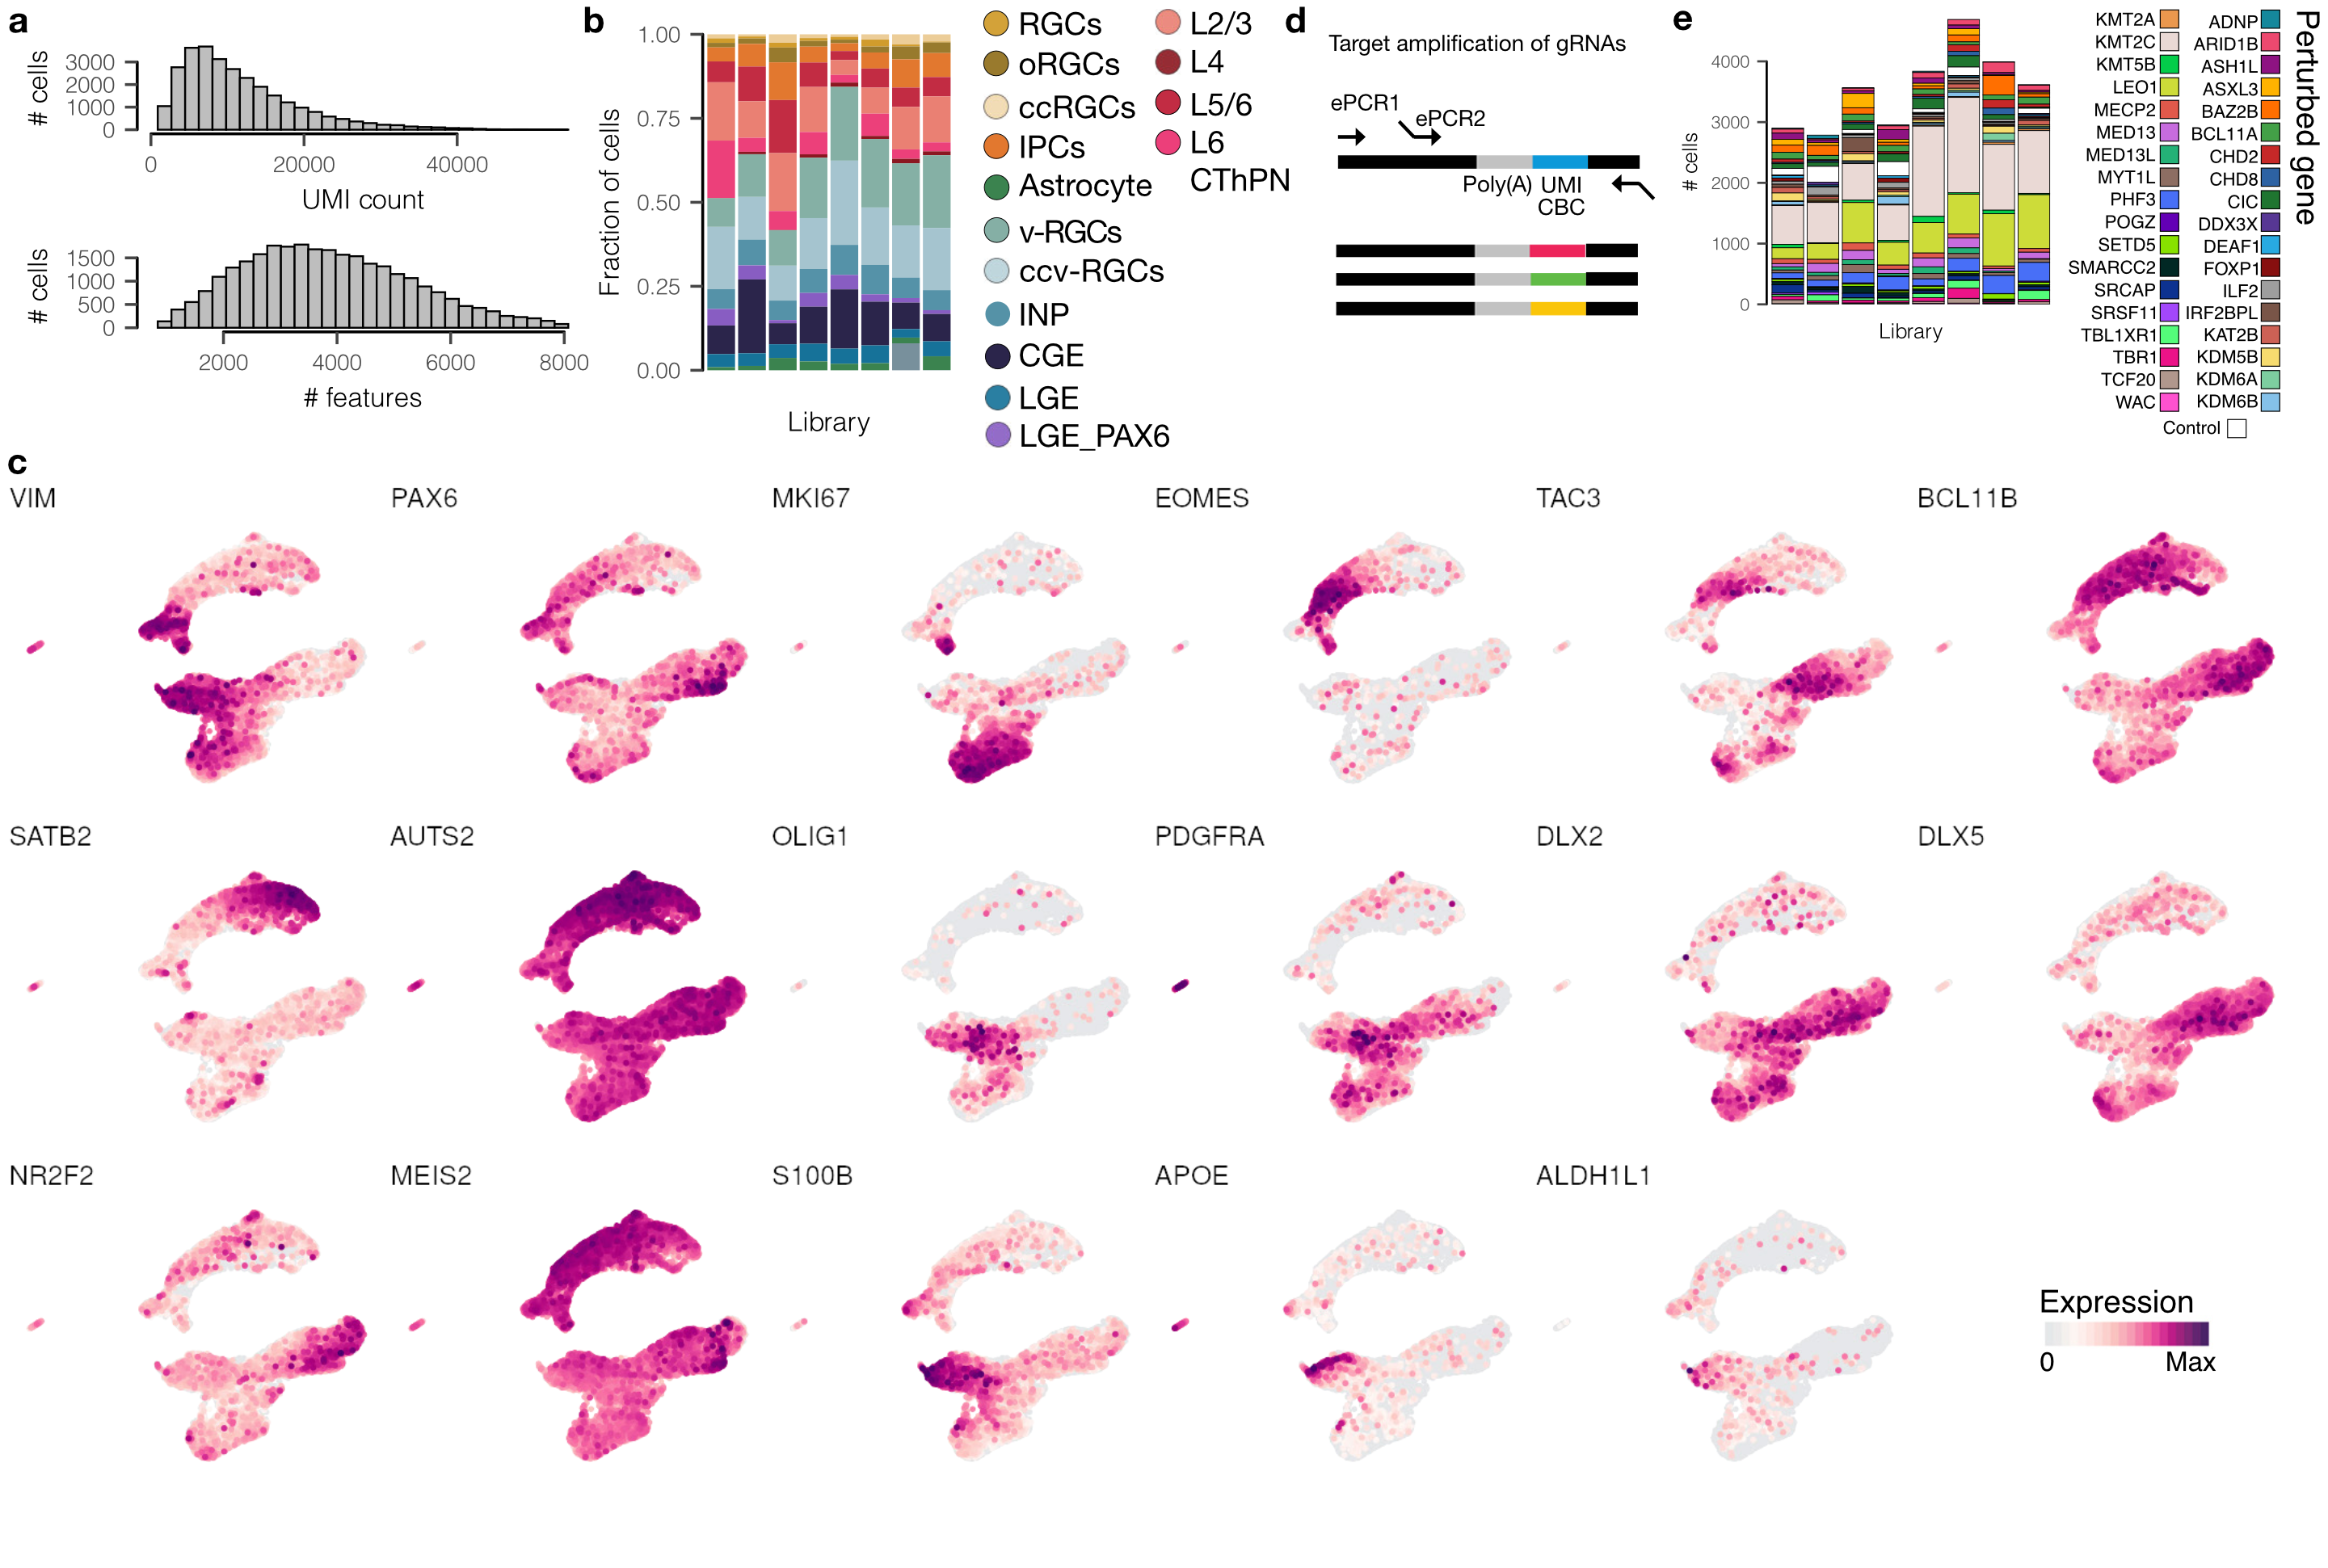
\includegraphics[width=\textwidth]{figures/asd/Figure_S5}
    \label{fig:asdS5}
    \caption{\textbf{Cell type and gRNA composition of scRNA-seq libraries.} 
    a, Histograms showing UMI count and number of detected features in the QC-controlled scRNA-seq dataset. b, Cell type compositions for each 10X library. In total 8 libraries (31 cerebral organoids) are processed and sequenced. c, Feature plots showing expression of marker genes on a UMAP embedding. d, Target amplification with hemi-nested emulsion PCR (ePCR) used to recover gRNA information. e, Bar plot shows numbers of recovered cells with assigned gRNAs for each library.}
\end{figure}



\begin{figure}[h!]
    \centering
	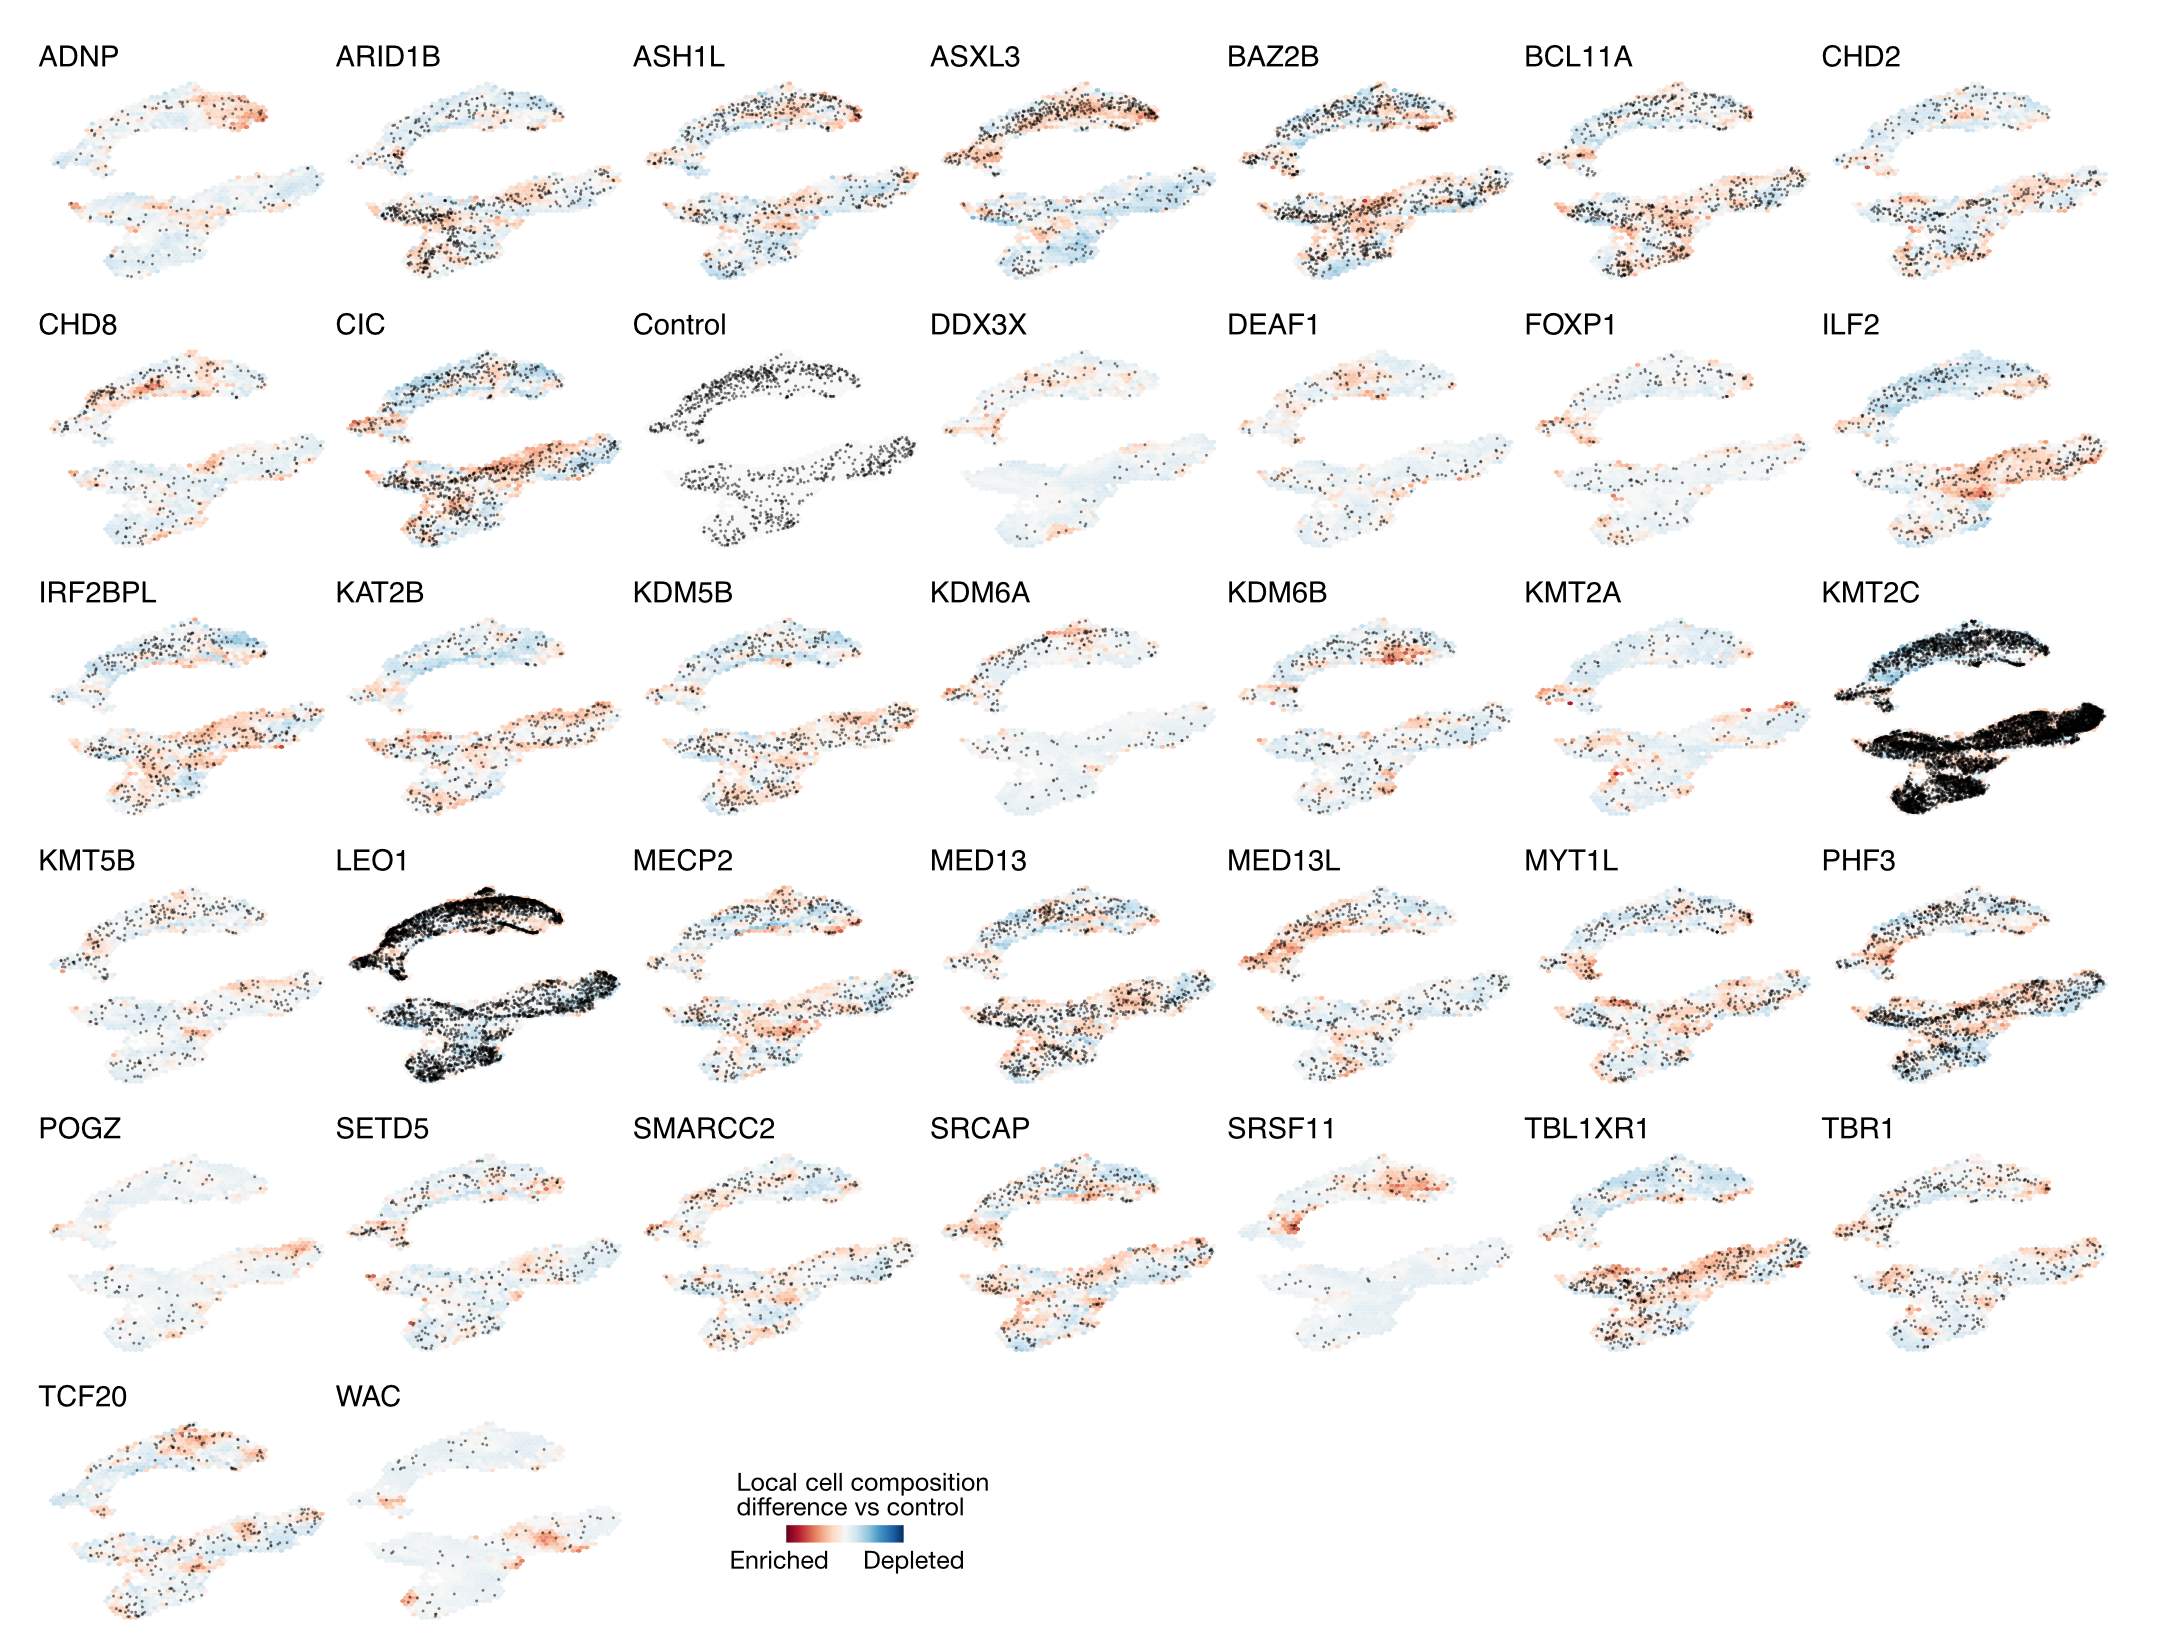
\includegraphics[width=\textwidth]{figures/asd/Figure_S6}
    \label{fig:asdS6}
    \caption{\textbf{Cell type compositional changes caused by ASD gene perturbations.} 
    UMAP embeddings show single cell distribution for each perturbed gene. Local cell composition differences of perturbation versus control indicated by red (enrichment) or blue (depletion).}
\end{figure}



\begin{figure}[h!]
    \centering
	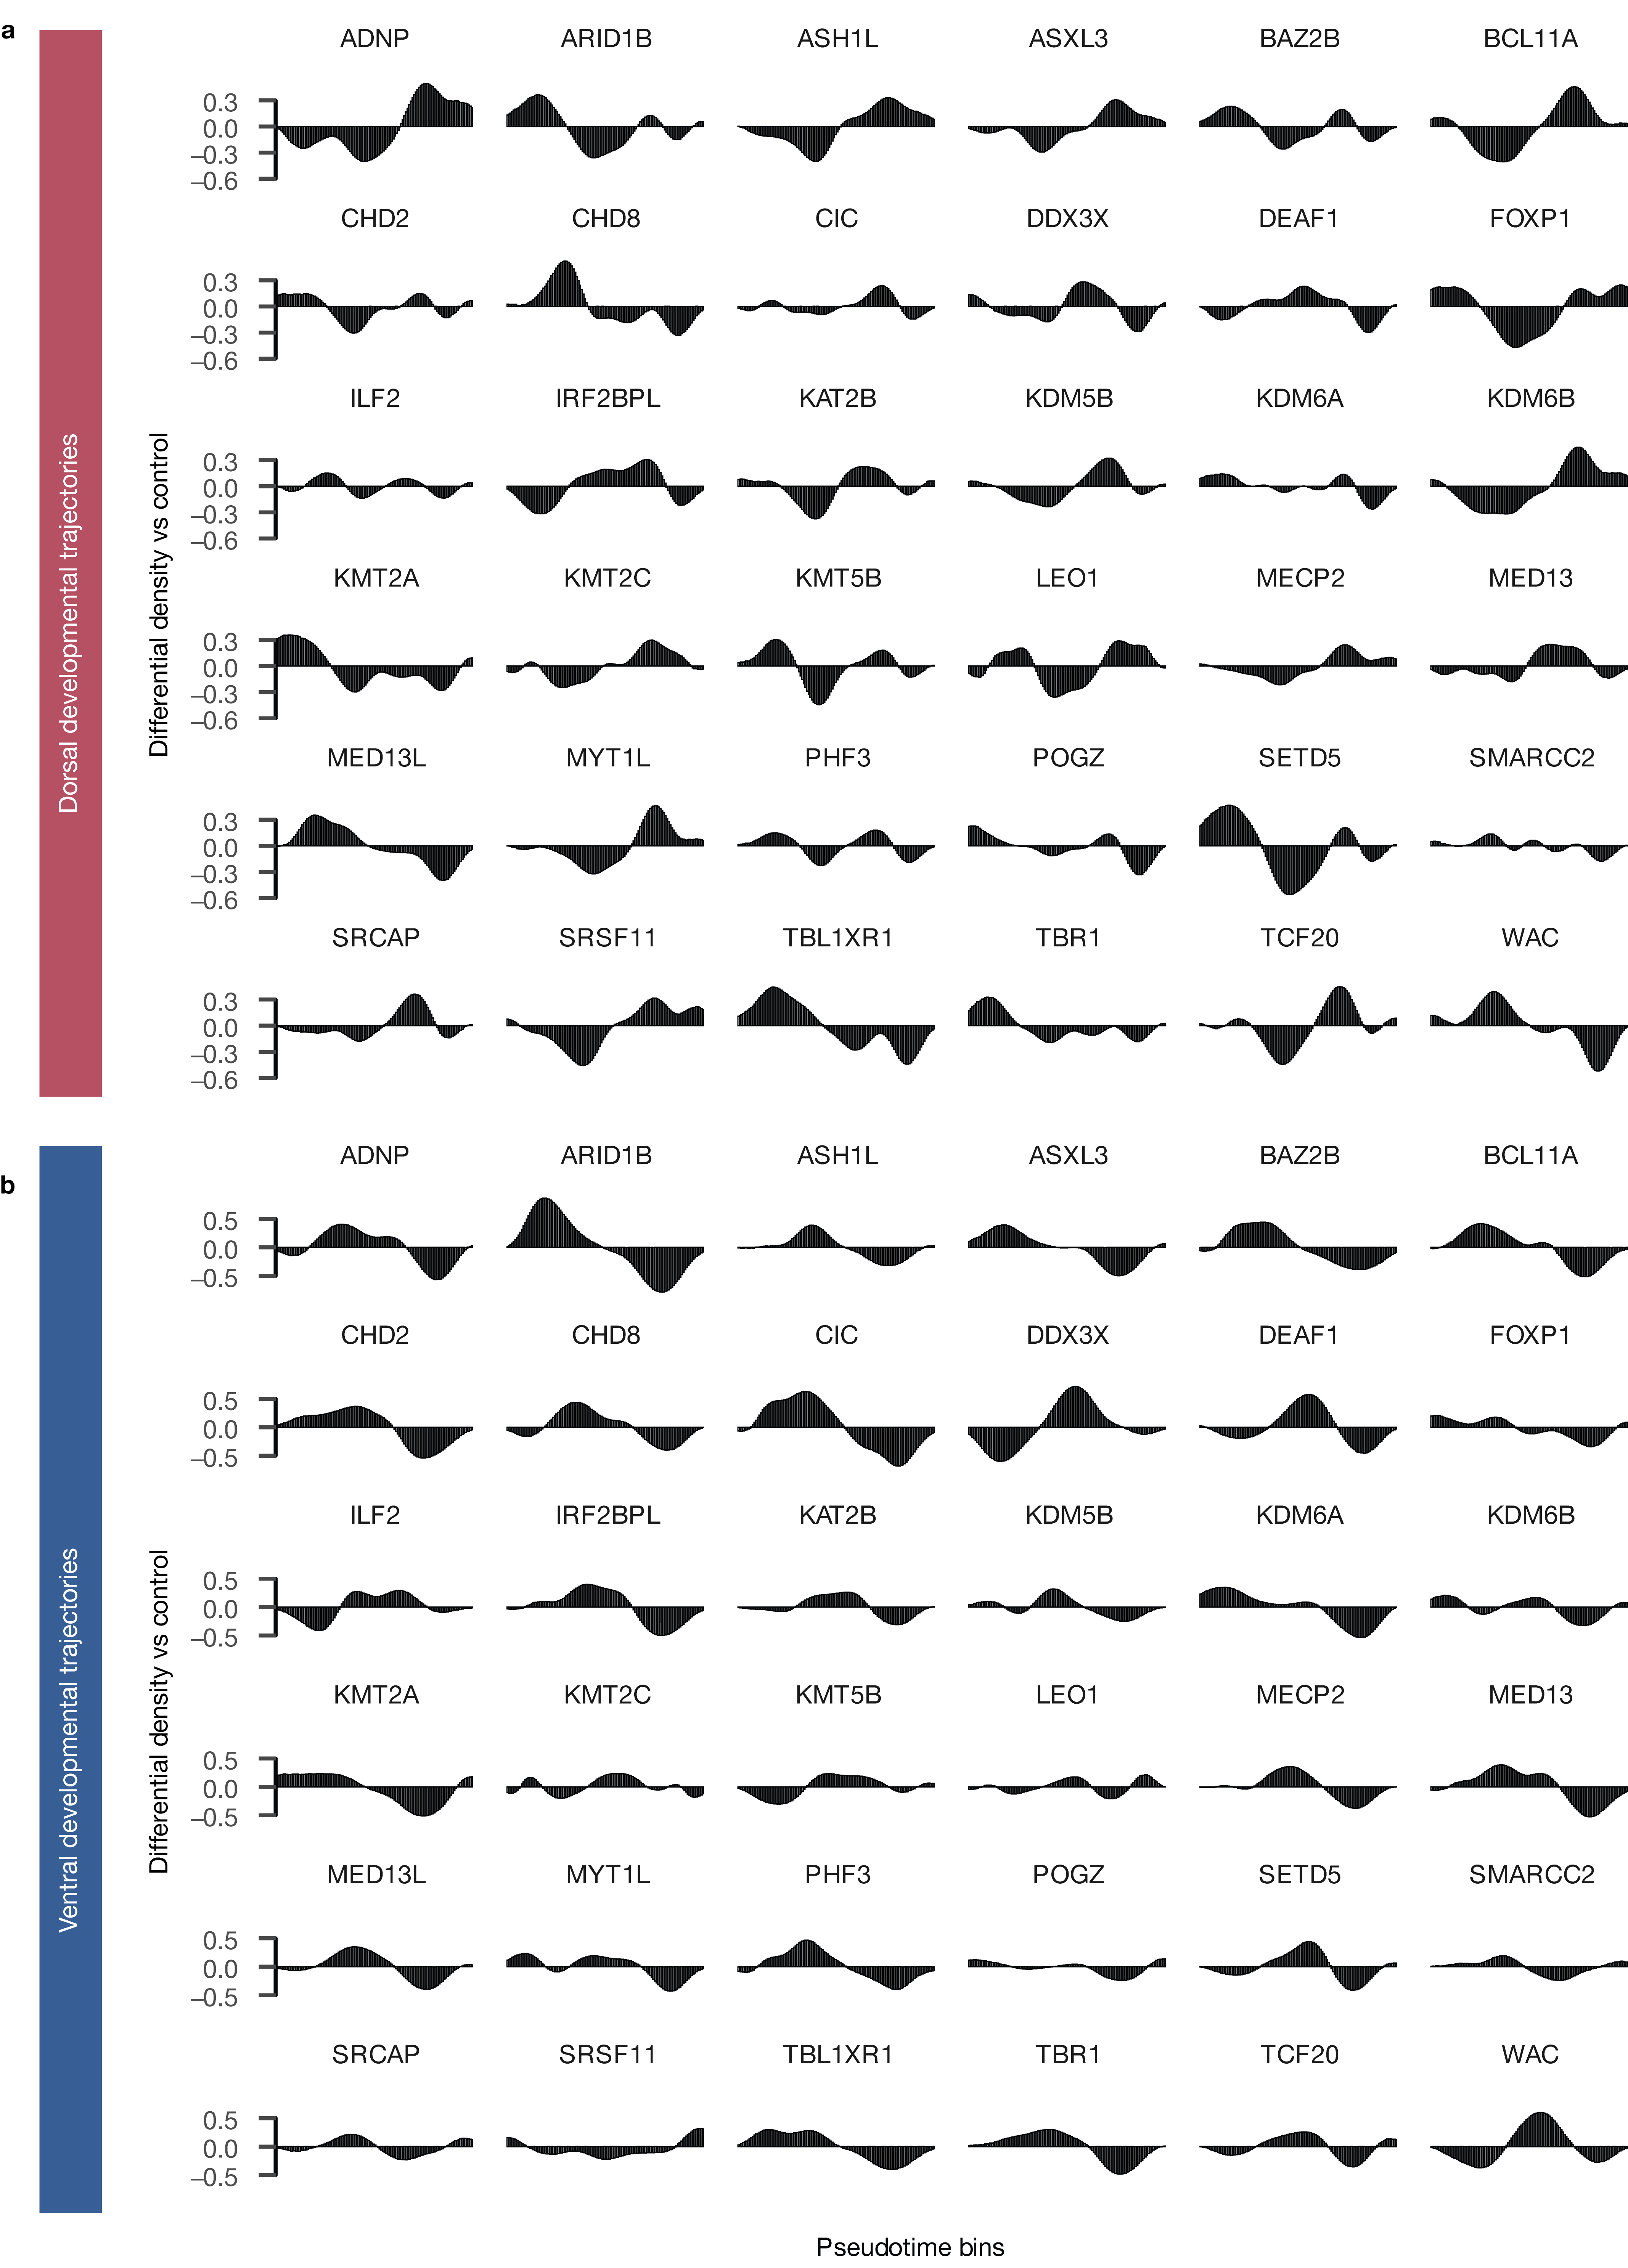
\includegraphics[width=\textwidth]{figures/asd/Figure_S7}
    \label{fig:asdS7}
    \caption{\textbf{Developmental process-specific effects of ASD gene perturbations.} 
    Differential cell density along a binned pseudo-temporal axis of perturbations versus control for each gene perturbation. Plots are separated by dorsal and ventral telencephalon trajectories.}
\end{figure}



\begin{figure}[h!]
    \centering
	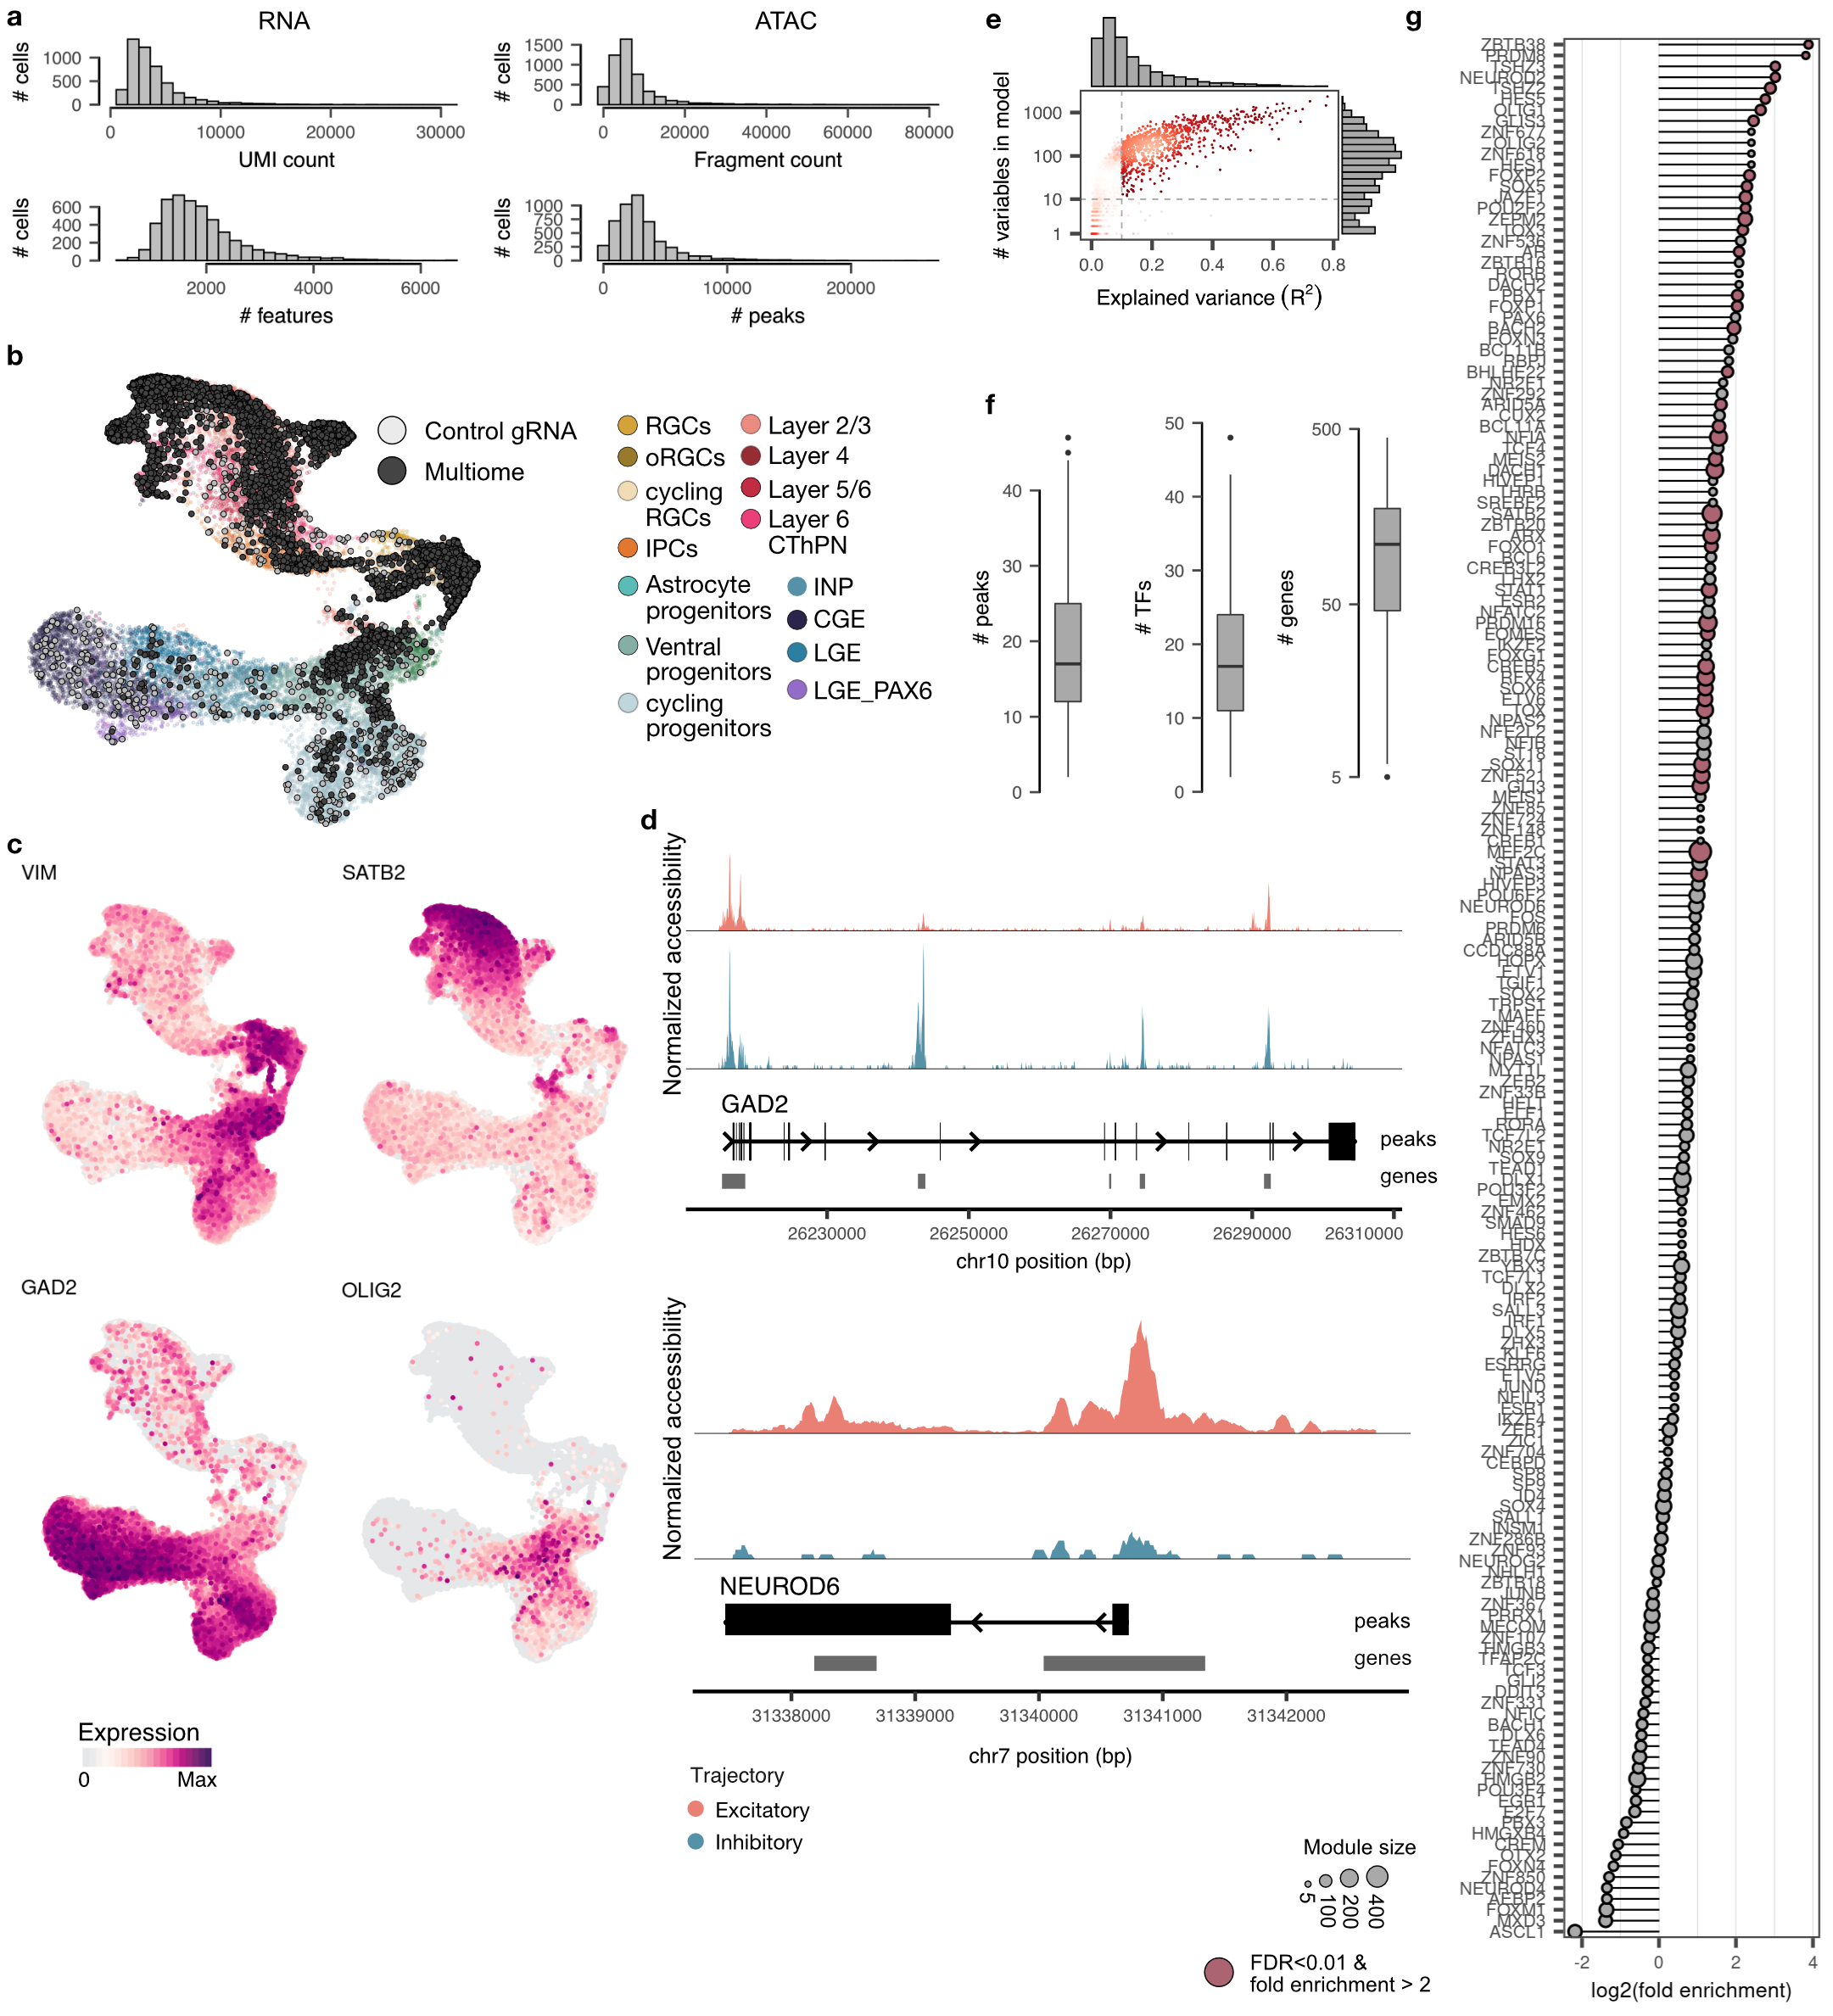
\includegraphics[width=\textwidth]{figures/asd/Figure_S8}
    \label{fig:asdS8}
    \caption{\textbf{Quality control and GRN inference from the single-cell multiome dataset.} 
    a, Histograms showing UMI count and number of detected features for RNA as well as fragment count and number of detected peaks for ATAC. b, UMAP embedding showing multiome data (black) integrated with the CHOOSE dataset. Multiome data were used in conjunction with the control cells from the CHOOSE dataset (grey) to infer the GRN with Pando. c, Feature plots showing expression of marker genes on the UMAP embedding. d, Genomic tracks showing accessible peaks in the proximity of GAD2 (ventral marker) and NEUROD6 (dorsal marker). e, Density scatter plot histograms showing the distributions of explained variance (x) and number of variables (y) in the fitted models for GRN construction. Dashed lines indicate the thresholds used for model selection. f, Boxplots showing the distribution of peaks (left) and TFs assigned per gene (middle), and number of genes assigned per TF (right) in the inferred GRN. g, Lolliplot showing the enrichment of ASD-associated genes from SFARI in inferred TF modules. Red color indicates an FDR-corrected Fisher-test p-value of <0.01. Dot size indicates the total number of genes in the module.}
\end{figure}



\begin{figure}[h!]
    \centering
	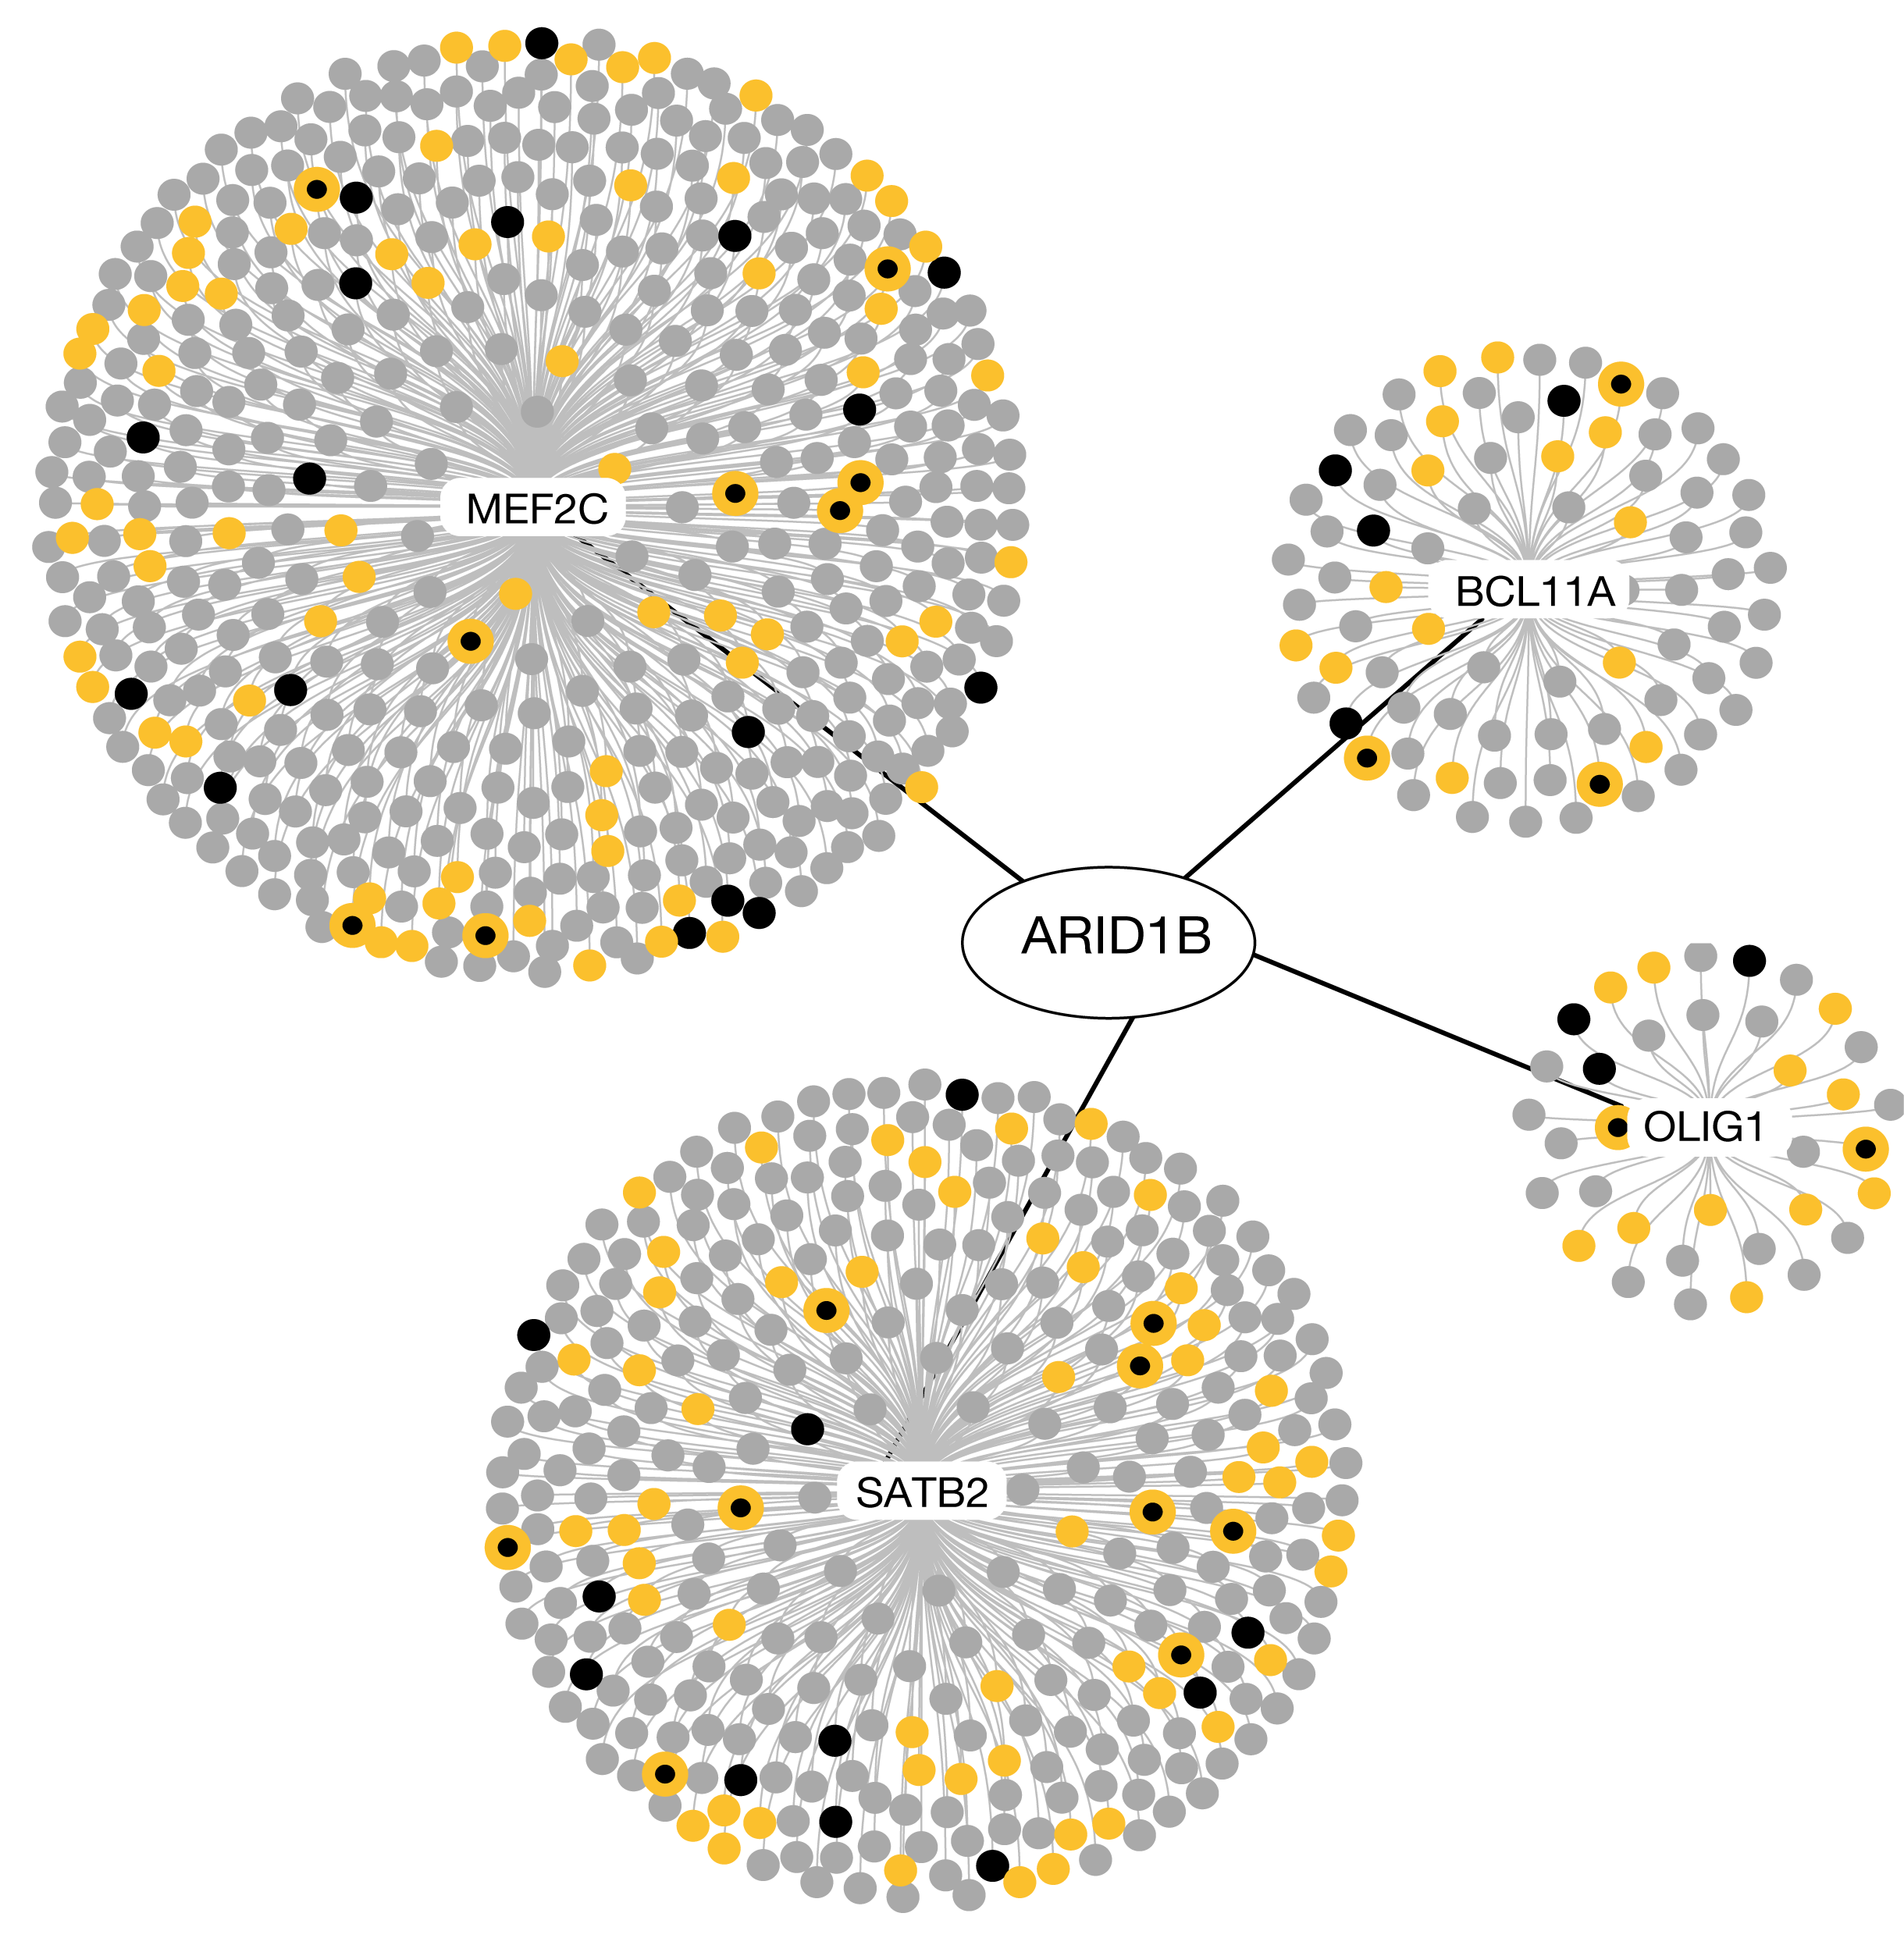
\includegraphics[width=\textwidth]{figures/asd/Figure_S9}
    \label{fig:asdS9}
    \caption{\textbf{ARID1B perturbation-induced DEGs are enriched in the OLIG1 regulatory module.}  
    Graph representation of MEF2C, BCL11A, SATB2, and OLIG1 TF modules, which are most strongly enriched in ARID1B DEG (Fisher exact test p-value < 0.01, top 4 odds ratio). The targets highlighted in yellow are SFARI genes, and the targets highlighted in black are TF modules enriched in SFARI genes. }
\end{figure}



\begin{figure}[h!]
    \centering
	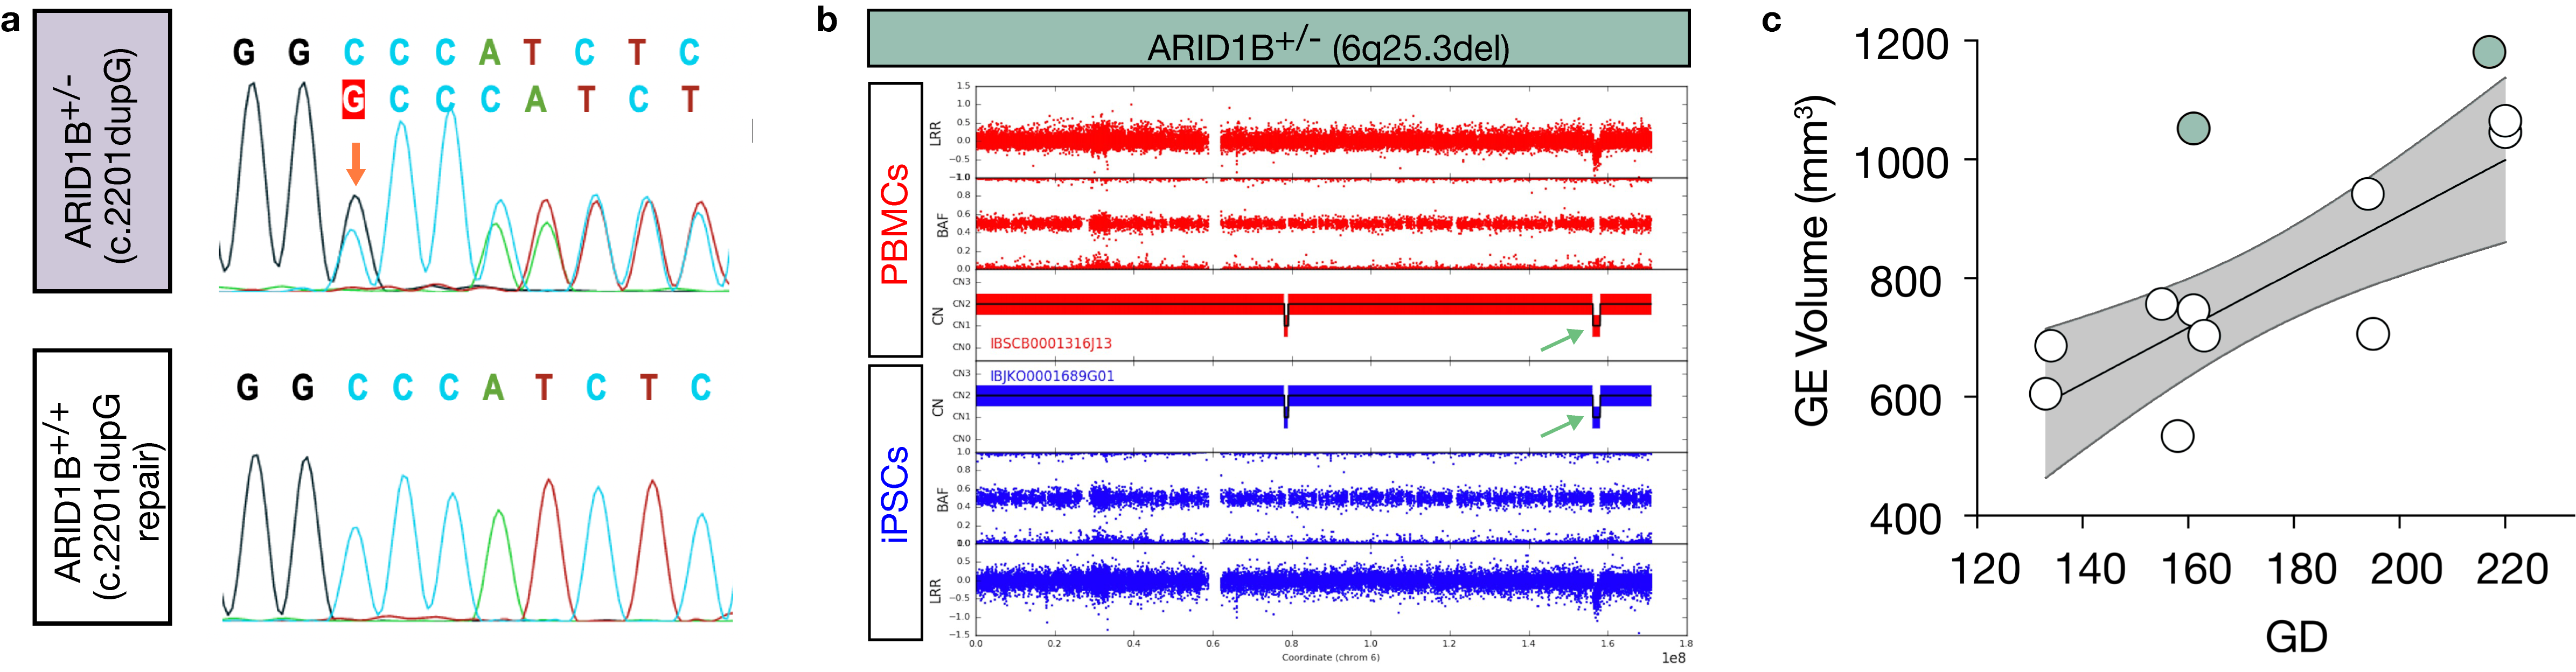
\includegraphics[width=\textwidth]{figures/asd/Figure_S10}
    \label{fig:asdS10}
    \caption{\textbf{An ARID1B patient had enlarged ganglionic eminence.}  
    a, Top, sanger sequencing showing a duplication mutation (red arrow) identified in one of the alleles of patient 1. Bottom, sanger sequencing showing the mutation was repaired and this cell line is used as an isogenic control. Sequencing was done on fragments amplified from genomic DNA extracted from the two iPSC lines.  b, SNP array genotyping of PBMCs and iPSCs from patient 2 shows a microdeletion (dark green arrow) identified on chromosome 6. c, Dot plot of the GE (LGE and CGE) volume of patient 2 (dark green circles) at two gestation stages. The white circles represent age-matched controls. A simple linear regression model was constructed using data from all controls. The gray area represents the 95\% confidence interval.}
\end{figure}

